% !TeX root = RJwrapper.tex
\title{\pkg{LUCIDus}: An R Package For Implementing Latent Unknown Clustering By Integrating Multi-omics Data (LUCID) With Phenotypic Traits}
\author{by Yinqi Zhao, Qiran Jia, Jesse A. Goodrich, David V. Conti}

\maketitle

\begin{abstract}
Many studies are leveraging current technologies to obtain multiple omics measurements on the same individuals. These measurements are usually cross-sectional and methods developed and commonly used focus on omic-integration at a single time point. More unique, and a growing area of interest, are studies that leverage biology or the temporal sequence of measurements to relate long-term exposures or germline genetics to intermediate measures capturing transitional processes that ultimately result in an outcome. In this context, we have previously introduced an integrative model named Latent Unknown Clustering by Integrating multi-omics Data (LUCID) aiming to distinguish unique effects of environmental exposures or germline genetics and informative omic effects while jointly estimating subgroups of individuals relevant to the outcome of interest. This multiple omics analysis consists of early integration (concatenation of omic layers to estimate common subgroups); intermediate integration (omic-layer-specific estimation of subgroups that are all related to the outcome); late integration (omic-layer-specific estimation of subgroups that are then inter-related by $a priori$ structures). In this article, we introduce \pkg{LUCIDus} version 3, an R package to implement the LUCID model. We review the statistical background of the model and introduce the workflow of \pkg{LUCIDus}, including model fitting, model selection, interpretation, inference, and prediction. Throughout, we use a realistic but simulated dataset based on an ongoing study, the Human Early Life Exposome Study (HELIX) to illustrate the workflow.
\end{abstract}

%--------------------- section 1: introduction --------------------
\section{Introduction} \label{sec1}

The rapid advancement in high throughput technology has made it possible to measure multiple omics (referred to as ``multi-omics'') data on the same person in many cohort studies. These data sets include DNA genome sequences \citep{goodwin2016coming}, RNA expression data \citep{ozsolak2011rna}, metabolites in biofluids \citep{beger2013review}, proteins in cell or tissue \citep{aslam2017proteomics}, as well as chemical exposures in the environment \citep{wild2005complementing}.For example, the Human Early-Life Exposome project (HELIX) measured molecular omics signatures including RNA expression data, metabolites, plasma proteins etc. from 1300 children at the age of 6-11 in six European countries \citep{vrijheid2014human}. Guided by biology or the temporal sequence of measurements, these studies often share a common structure that relates germline genetics or environmental exposures to intermediate factors capturing transitional processes that ultimately result in an outcome. While these suspected causal pathways can be measured with current omic technology, the analysis often focuses on cross-sectional relationships using cluster analysis or models focused on feature selection. This is in part due to the analytic and computational challenges resulting from the complex structure of the data collected from various sources, the limited sample size, and the high-dimensionality of multi-omics information \citep{tini2019multi}. Existing methods do not consider risk factors that precede the omic measurements and link those factors with disease or trait outcomes while using multi-omics data to characterize the underlying mechanism. Thus, there is a great need to develop and easily implement approaches leveraging these mediating relationships or latent structures for the integration of multi-omics data \citep{subramanian2020multi}. 

Conventional analysis tools range from clustering approaches to variable selection approaches \citep{gonzalez2019omic}. Clustering is a fundamental method for analyzing both single omic and multi-omics data \citep{rappoport2018multi}. Clustering aims to divide observations into several groups (called clusters) such that observations within a group are similar while samples in different groups are dissimilar. Clustering has many important applications in the field of biological science and medicine, such as defining gene sets \citep{hejblum2015time}, identifying subtypes of cancer and performing diagnostic prediction \citep{curtis2012genomic, khan2001classification}, defining cell types in flow cytometry and scRNAseq experiments \citep{chan2008statistical, hejblum2019sequential, prabhakaran2016dirichlet}, and estimating protein localization \citep{crook2018bayesian}. Conventional clustering methods applied to multi-omics data either concatenate multiple datasets (often called early integration) or analyze each dataset independently (i.e. late integration). However, both approaches fall short of adequately capturing the variation across omic levels or reflecting the heterogeneity of the integrated datasets. To overcome these limitations, several specific integrated clustering methods for analyzing multi-omics data are available in the community. \citet{pierre2020clustering} conducted a thorough review comparing 13 unsupervised methods for multi-omics data integration via clustering. Methods include SGCCA \citep{tenenhaus2014variable}, SNF \citep{wang2014similarity}, iCluster plus \citep{mo2013pattern} etc. Building upon the foundation of Principal Component Analysis (PCA), Joint and Individual Variation Explained (JIVE) conducts integrated clustering of multi-omics data via a variance decomposition framework to summarize information across multiple omic layers. \citep{lock2013joint}. Within the Bayesian framework, \citet{kirk2012bayesian} proposed an unsupervised approach, Bayesian correlated clustering, that simultaneously models each omic layer via a mixture model while considering the correlation between each model. In a similar fashion, Bayesian consensus clustering can flexibly describe the dependency and the heterogeneity of the multi-omics data \citep{lock2013bayesian}. An alternative approach to clustering includes dimension reduction or variable selection to reduce noise, improve model interpretability, and avoid problems with overfitting. For example, the least absolute shrinkage and selection operator (LASSO) induces sparsity in model coefficients based on $L_1$ norm regularization \citep{tibshirani1996regression}. An extension of LASSO, Group LASSO, allows for variable selection on both individual and pre-specified grouped variables \citep{yuan2006model}. $L_1$ norm regularization is integrated into many clustering approaches to reduce data dimensionality, such as SGCCA and iCluster plus. Extensions of variable selection approaches exist for mediation as well and include both high-dimensional and latent variable approaches. HIMA first implements pre-screening of the high-dimensional mediators and then utilizes a LASSO-type penalty to obtain a sparse solution \citep{zhang2016estimating}, while BAMA is a Bayesian shrinkage approach that employs continuous shrinkage priors on the key coefficients to select active mediators with large effects only \citep{song2020bayesian}. Both \citet{albert2016causal} and \citet{derkach2019high} proposed statistical models within the causal mediation framework that summarize the information from high-dimensional multi-omics data into a latent variable to facilitate interpretation. 

In the context of linking multi-omics to health outcomes and identifying key omic features that drive the outcomes, \citet{singh2019diablo} proposed Data Integration Analysis for Biomarker discovery using Latent cOmponents (DIABLO), which extends the unsupervised sGCCA to a supervised framework. DIABLO achieves summarizing common information across different omic layers and conducting variable selection while discriminating the outcome of interest. Nonetheless, DIABLO fails to take into account the impact of risk factors related to the outcome and their interplay with multi-omics data. Finally, \citet{peng2020latent} proposed a model called Latent Unknown Clustering by Integrating multi-omics Data (LUCID) that incorporates both clustering and variable selection to distinguish unique effects of germline genetics or environmental exposures and informative omic effects while jointly estimating subgroups of individuals relevant to the outcome of interest. LUCID is a novel 'quasi-mediation' approach that uses latent variable analysis to estimate subgroups of individuals characterized by key omic factors and with differential association to the outcome and exposures. They demonstrated the performance of LUCID through extensive simulation studies and real data applications to highlight the integration of genomic, exposomic, and metabolomic data. \CRANpkg{LUCIDus}, the R package to implement the LUCID model, provides an integrated clustering framework and has numerous downloads (around 19,000 times since it was first introduced according to \CRANpkg{dlstats} \citep{yu2022dlstats}). It has also been applied in several environmental epidemiological studies \citep{jin2020perfluoroalkyl, stratakis2020prenatal, matta2022associations}. In this paper, we introduced \pkg{LUCIDus} version 3, a major update and enhancement from the original release \citep{LUCIDus}. To account for the heterogeneity of the integrated datasets based on the study design, \pkg{LUCIDus} version 3 incorporates three integration strategies into the LUCID framework: (1) Early integration (Figure \ref{fig1} (a)) concatenates all multi-omics data matrices into a single matrix prior to model estimation; (2) Intermediate integration (Figure \ref{fig1} (b)) estimates latent clusters for each omic layer and the resulting clusters are then modeled in parallel in a joint model linking exposures and the outcome; and (3) late integration (Figure \ref{fig1} (c)) in which each omic layer is used to estimate omic-specific clusters that are then linked via $ a priori$ relationships with each other and the exposure and outcome. \pkg{LUCIDus} version 3 also includes model selection, model visualization, and inference based on bootstrap resampling. It also incorporates an integrated imputation approach to deal with missingness in multi-omics data. The paper is organized as follows: we first briefly introduce the statistical model of LUCID; we then go through the details of functions in the \pkg{LUCIDus} package; we illustrate the workflow of fitting LUCID models by using a dataset simulated based on real cases from the HELIX study \citep{vrijheid2014human, maitre2022state}.


%--------------------- section 2: model and software --------------------
\section{Model and software} \label{sec2}

%--------------------- section 2.1: overivew of lucid --------------------
\subsection{Overview of the original LUCID model (early integration)} \label{sec2.1}

\begin{figure}
    \centering
    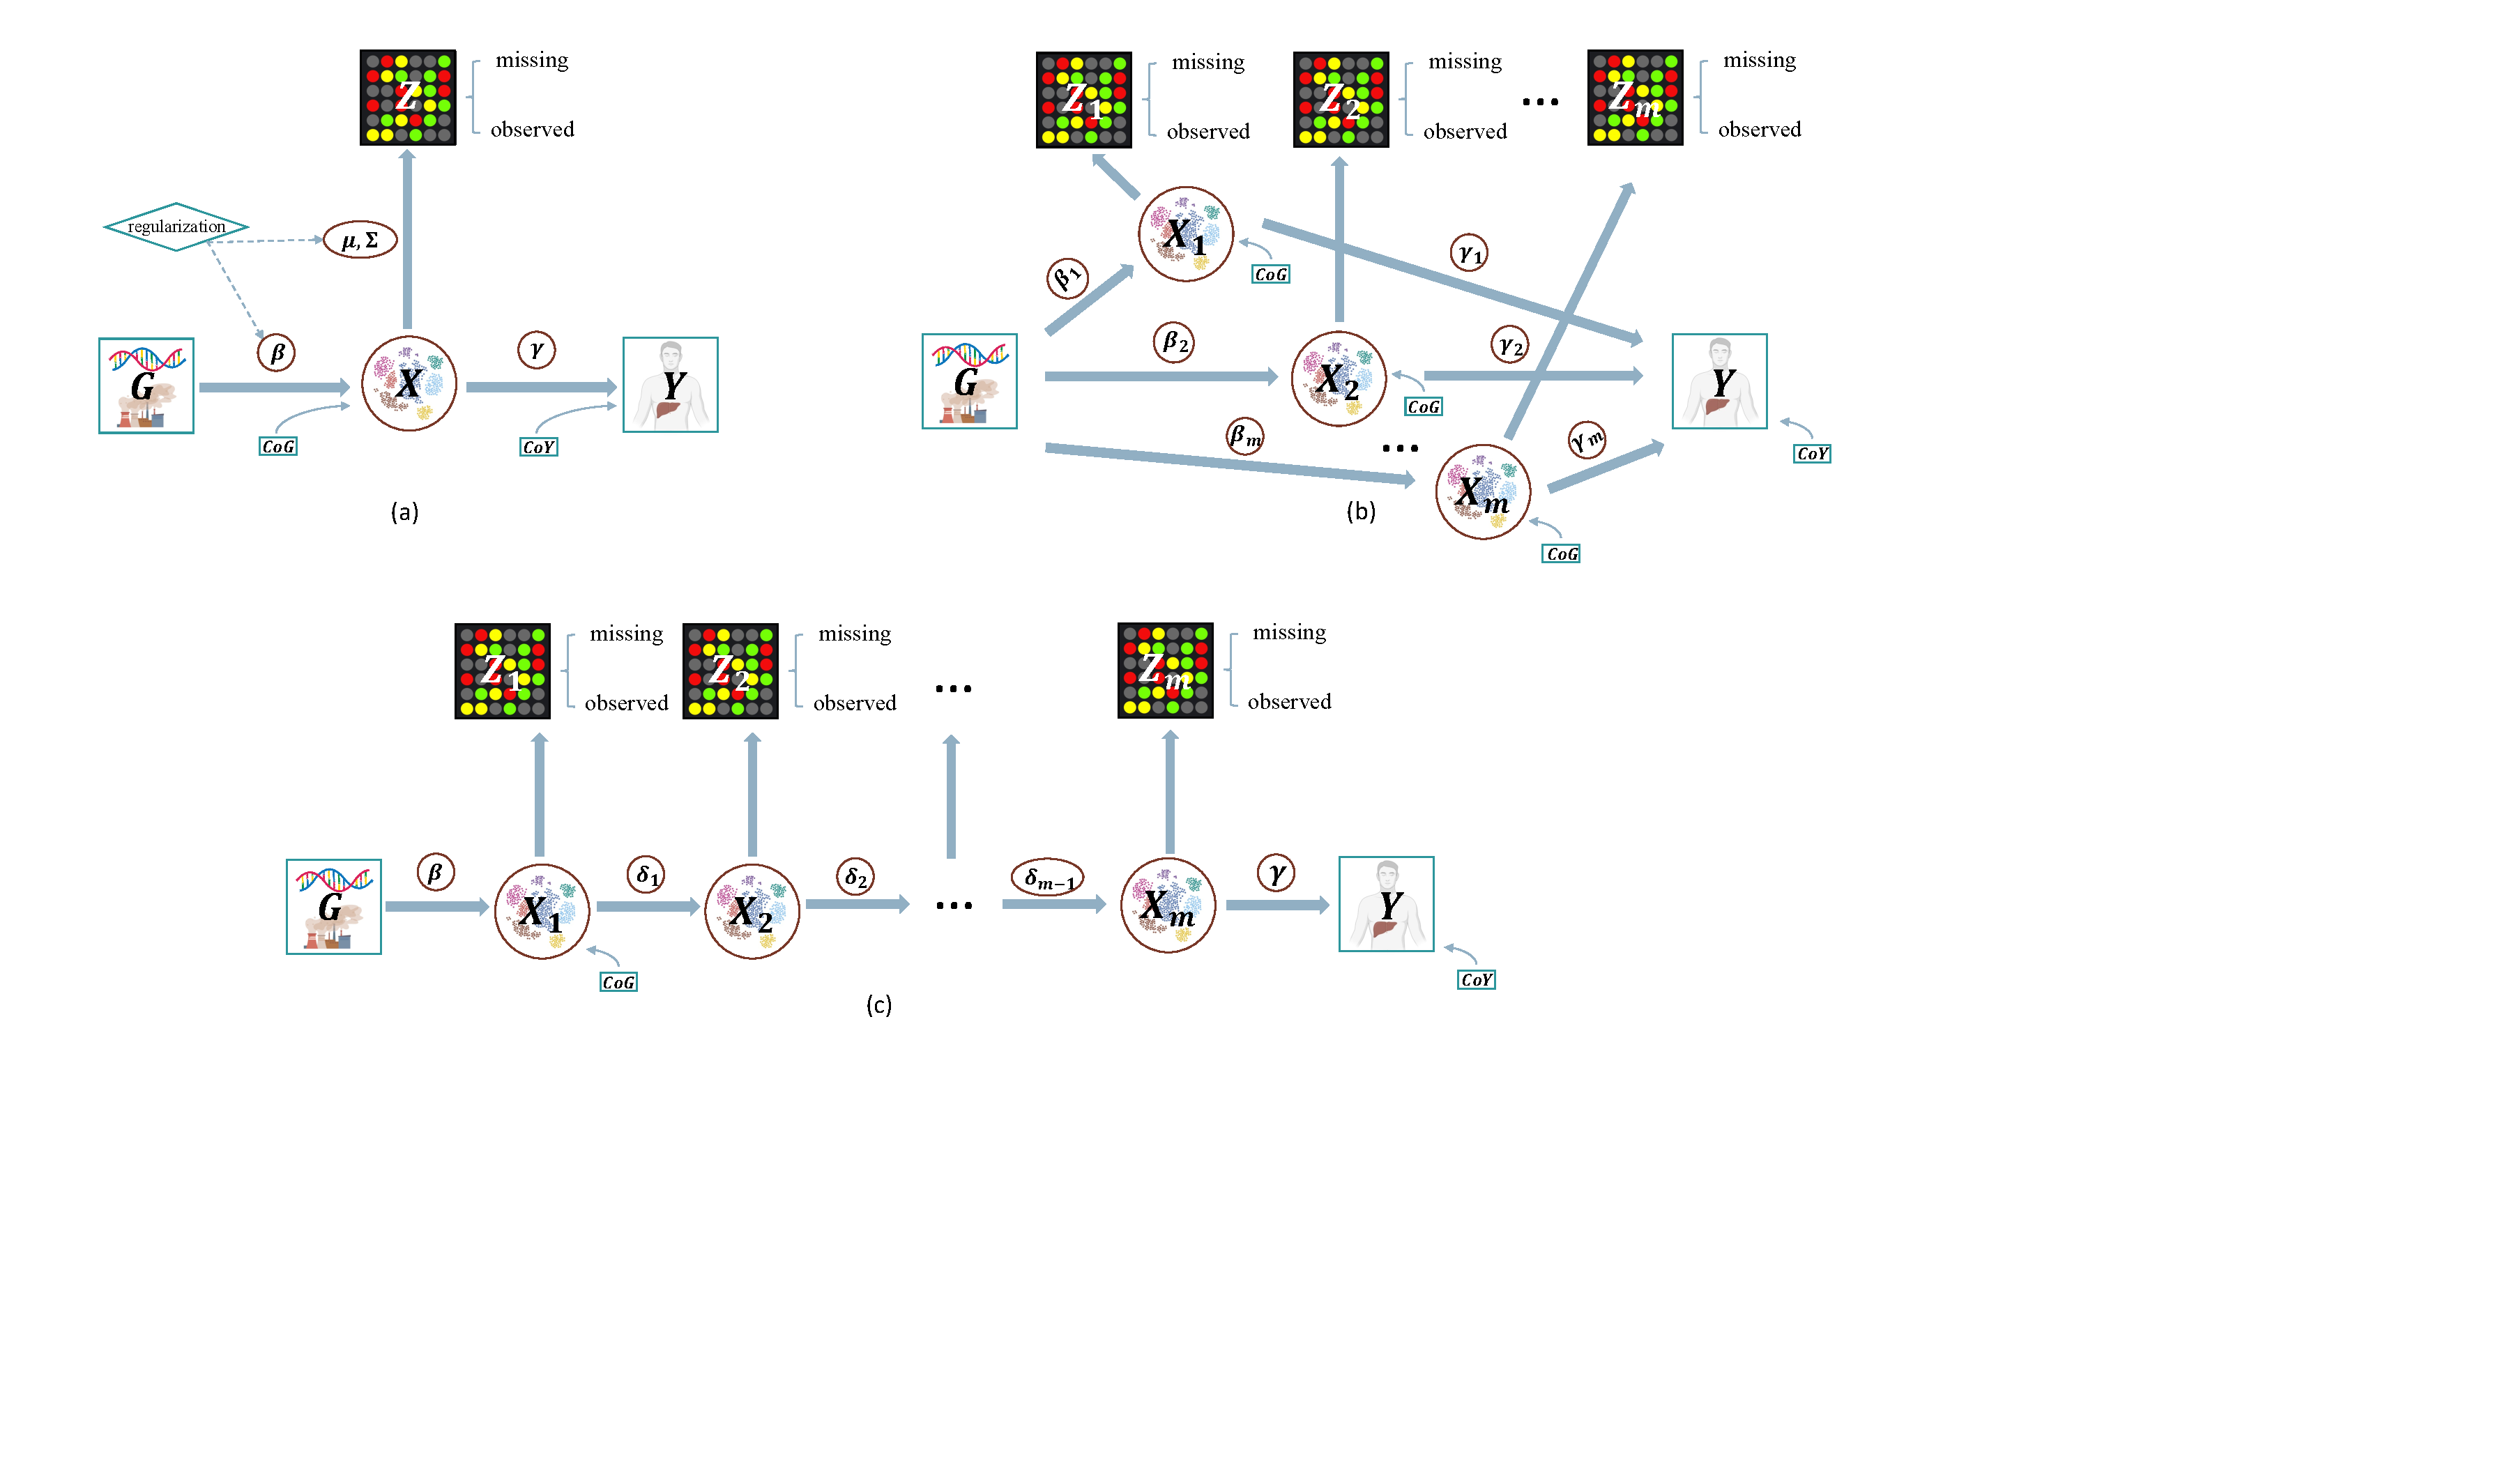
\includegraphics[scale = 0.31]{figures/fig1.pdf}
    \caption{Three DAGs represent how three different types of the LUCID model integrate genetic/environmental exposures ($\bm G$), other multi-omics data ($\bm Z$), and the phenotype trait ($\bm Y$). (a) LUCID early integration; (b) LUCID in parallel; (c) LUCID in serial. The squares represent observed data, the circles represent unobserved latent variables (clusters) and model parameters, and the diamond refers to $L_1$ penalty terms for regularization for (a). $\bm {CoG}$ and $\bm {CoY}$ represent covariates to be adjusted in the LUCID model. Missingness is allowed in multi-omics data. $\bm Z$ is divided into subsets of observations with complete measurements and observations with missingness. For (b) and (c), $\bm Z$ is partitioned into $m$ layers.}
    \label{fig1}
\end{figure}

In the LUCID model, genomic/exposomic exposures $\bm G$, other multi-omics data $\bm Z$, and phenotype trait $\bm Y$ are integrated through a latent categorical variable $\bm X$. To model the complex correlation structure between each layer of the multi-omics data, we propose three types of LUCID models based on different integration strategies: (1) LUCID early integration; (2) LUCID in parallel or intermediate integration; and (3) LUCID in serial or late integration. Figure \ref{fig1} illustrates the joint relationship between $\bm G$, $\bm Z$, $\bm X$, and $\bm Y$ for each LUCID model. We will discuss LUCID in parallel and LUCID in serial in detail under Sections \nameref{sec_parallel} and \nameref{sec_serial} as two extensions, and here we focus on LUCID early integration. Because $\bm X$ is an unobserved categorical variable, each category of $\bm X$ is interpreted as a latent cluster in the data, jointly defined by $\bm G$, $\bm Z$, and $\bm Y$. Let $\bm G$ be a $N \times P$ matrix with columns representing genetic/environmental exposures, and rows representing the observations; $\bm Z$ be a $N \times M$ matrix of omics data (for example, gene expression data, DNA methylation profiles, and metabolomic data, etc.) and $\bm Y$ be a $N$-length vector of phenotype trait. We further assume $\bm G$, $\bm Z$, and $\bm Y$ are measured through a prospective sampling procedure so we do not model the distribution of $\bm G$. All three measured components ($\bm G$, $\bm Z$, and $\bm Y$) are linked by a latent variable $\bm X$ consisting of $K$ categories. The directed acyclic graph (DAG) in Figure \ref{fig1} (a) implies the distributions of $\bm X$ given $\bm G$, $\bm Z$ given $\bm X$ and $\bm Y$ given $\bm X$ are conditionally independent with each other. Let $f(\cdot)$ denote the probability mass functions (PMF) for categorical random variables or the probability density functions (PDF) for continuous random variables. The joint log-likelihood of the LUCID model is constructed as:
\begin{equation}
    \begin{aligned}
         \log L(\bm{\Theta}) & = \sum_{i = 1}^N \log f(\bm{Z}_i, Y_i|\bm{G}_i;\bm{\Theta}) \\
         & = \sum_{i = 1}^N \log \sum_{j = 1}^K f(X_i = j| \bm{G}_i; \bm{\Theta}) f(\bm{Z}_i| X_i = j; \bm{\Theta}) f(Y_i|X_i = j; \bm{\Theta})
    \end{aligned}
    \label{eq1}
\end{equation}
where $\bm \Theta$ is a generic notation for all parameters in the LUCID model.

Since $\bm X$ is a discrete variable with $K$ categories, we assume $\bm X$ follows a multinomial distribution conditioning on $\bm G$, denoted by the softmax function $S(\cdot)$. We assume omics data $\bm Z$ follows a multivariate Gaussian distribution conditioning on $\bm X$, denoted by $\phi(\bm{Z}|\bm{X} = j; \bm{\mu}_j, \bm{\Sigma}_j)$, where $\bm{\mu}_j$ and $\bm{\Sigma}_j$ are cluster-specific mean and variance-covariance matrix for $\bm{Z}$. For illustrative purposes, we assume $\bm Y$ is a continuous outcome following a univariate Gaussian distribution, denoted by $\phi(\bm {Y}|\bm{X} = j; \gamma_j, \sigma_j^2)$ ($\gamma_j$ and $\sigma_j^2$ are also interpreted as the cluster-specific mean and variance for effect of $\bm{X}$ on $\bm{Y}$). Similar development for a binary outcome is detailed in \citep{peng2020latent}. Because the latent cluster $\bm X$ is unobserved, the maximum likelihood estimates (MLE) of the parameters associated with the LUCID model based on Equation \ref{eq1} are not readily estimated. Therefore, we use the Expectation-Maximization (EM) algorithm to obtain the MLE of model parameters. We define $I(X_i= j)$ as an indicator function representing that observation $i$ belongs to latent cluster $j$. Then, the log-likelihood function of model parameters in Equation \ref{eq1} becomes:
\begin{equation}
    \begin{aligned}
         \log L(\bm{\Theta}) & = \sum_{i = 1}^N \sum_{j=1}^K I(X_i = j) \left( \log S(X_i = j| \bm{G}_i; \bm{\Theta}) + \log \phi(\bm{Z}_i| X_i = j; \bm{\Theta}) + \log \phi (Y_i|X_i = j; \bm{\Theta}) \right)
    \end{aligned}
    \label{eq2}
\end{equation}

We denote the observed data as $\bm {D} = \{\bm {G}, \bm {Z}, \bm{Y}\}$, and define the responsibility $r$ as the inclusion probability (IP) of belonging to the latent cluster $j$ given observed data and current estimation of model parameters at iteration $t$, which is:
\begin{equation}
    \begin{aligned}
        r_{ij}^{(t)} & = P(X_i = j|\bm{D}; \bm{\Theta}^{(t)}) \\
            & = \frac{S\left(X_i = j| \bm{G}_i; \bm{\beta}^{(t)}\right) \phi\left(\bm{Z}_i| X_i = j; \bm{\mu}_j^{(t)}, \bm{\Sigma}_j^{(t)}\right) \phi\left(Y_i|X_i = j; \gamma_j^{(t)}, \sigma^{2(t)}_j \right)}{\sum_{j = 1}^K S\left(X_i = j| \bm{G}_i; \bm{\beta}^{(t)}\right) \phi \left(\bm{Z}_i| X_i = j; \bm{\mu}_j^{(t)}, \bm{\Sigma}_j^{(t)}\right) \phi \left(Y_i|X_i = j; \gamma_j^{(t)}, \sigma^{2(t)}_j\right)}
    \end{aligned}
    \label{eq3}
\end{equation}

At each iteration $t$, in the E-step, we compute the expectation of the complete data likelihood, which is:
\begin{equation}
    \begin{aligned}
        Q(\bm{\Theta}|\bm{D}, \bm{\Theta}^{(t)}) = & \sum_{i=1}^N\sum_{j=1}^K r_{ij} \log S\left(X_i = j|\bm{G}_i;\bm{\beta}\right) + \sum_{i=1}^N\sum_{j=1}^K r_{ij} \log \phi(\bm{Z}_i|X_i = j;\bm{\mu}_j, \bm{\Sigma}_j) \\
        & + \sum_{i=1}^N\sum_{j=1}^K r_{ij} \log \phi\left(Y|X_i = j; \gamma_j, \sigma_j^2\right)
    \end{aligned}
    \label{eq4}
\end{equation}

In the M-step, we update parameter estimates by maximizing Equation \ref{eq4} in terms of $\bm \Theta$, which results in the following:
\begin{align}
    \bm \beta^{(t+1)} & = \arg \max_{\bm \beta} \sum_{i=1}^N \sum_{j=1}^K r_{ij}^{(t)} \log S(X_i = j| \bm G_i; \bm \beta_j) \label{eq5} \\
    \bm \mu_j^{(t+1)} & = \frac{\sum_{i=1}^N r_{ij}^{(t)}\bm Z_i}{\sum_{i=1}^N r_{ij}^{(t)}} \label{eq6} \\
    \bm \Sigma_j^{(t+1)} & = \frac{\sum_{i=1}^N r_{ij}^{(t)} \left(\bm{Z}_i - \bm{\mu}_j^{(t+1)} \right) \left(\bm{Z}_i - \bm{\mu}_j^{(t+1)} \right)^T}{\sum_{i=1}^N r_{ij}^{(t)}} \label{eq7} \\
    \gamma_j^{(t+1)} & = \frac{\sum_{i=1}^N r_{ij}^{(t)}Y_i}{\sum_{i=1}^N r_{ij}^{(t)}} \label{eq8} \\
    \sigma_j^{2(t+1)} & = \frac{\sum_{i=1}^N r_{ij}^{(t)} \left(Y_i - \gamma_j^{(t+1)} \right)^2}{\sum_{i=1}^N r_{ij}^{(t)}} \label{eq9}
\end{align}
Although maximization of $\bm \beta_j^{(t+1)}$ in Equation \ref{eq5} does not have a closed form solution, it is equivalent to fitting a multinomial logistic regression by treating $r_{ij}$ as the outcome and $\bm G_i$ as the exposure.

For \pkg{LUCIDus}, we include a more flexible geometric feature of latent clusters, such as volume, shape, and orientation determined by $\bm \Sigma_j$.  We use the parameterization of covariance matrices by means of an eigenvalue decomposition in the form below \citep{banfield1993model}:
\begin{equation}
    \bm \Sigma_j = \lambda_j \bm D_j \bm A_j \bm D_j^T \label{eq10}
\end{equation}
where $\lambda_j$ is a scalar, $\bm D_j$ is the orthogonal matrix of eigenvectors and $\bm A_j$ is a diagonal matrix whose values are proportional to eigenvalues. A detailed discussion of maximizing $\bm \Sigma_j$ parameterized by Equation \ref{eq10} is provided by \citet{celeux1995gaussian}. Their algorithm is implemented in the R package \CRANpkg{mclust} \citep{scrucca2016mclust} and we leverage \pkg{mclust} to update $\bm \Sigma_j$ in M-step at each iteration of EM algorithm for LUCID.

%--------------------- section 2.2: general workflow of lucid --------------------
\begin{table}[]
\begin{tabular}{p{0.25\textwidth}p{0.7\textwidth}}
\hline
\textbf{Main function}      & \textbf{Description} \\ 
\hline
\code{lucid()}              & Main function to fit LUCID models, specified by giving integrated data, a distribution of the outcome and the type of the LUCID model (early, parallel, serial). It also conducts model selection and variable selection for LUCID early integration and model selection for candidate models with different numbers of latent clusters for LUCID in parallel and LUCID in serial.\\
\code{summary()}     & S3 method for LUCID. Create tables to summarize a LUCID model.\\
\code{plot()}        & S3 method for LUCID. Visualize LUCID models through a Sankey diagram.\\
\code{boot\_lucid()}        & Derive confidence intervals based on bootstrap resampling.\\
\code{predict\_lucid()}     & Predict latent cluster assignment and outcome using integrated data.\\
\hline \hline
\textbf{Workhorse function} & \textbf{Description}\\
\hline
\code{estimate\_lucid()}         & Fit a LUCID model to estimate latent clusters by using integrated data.\\
\code{tune\_lucid()}        & It fits a series of LUCID models over different combinations of tuning parameters and determines an optimal model with the minimum BIC. \\ \hline
\end{tabular}
\caption{Functions in the \pkg{LUCIDus} package. \code{lucid()} calls \code{estimate\_lucid()} and \code{tune\_lucid()} in the backend. The two workhorse functions are not normally called directly, but they can be useful when a user wants to examine the model fitting process in more detail.}
\label{tbl1}
\end{table}

\begin{figure}[]
    \centering
    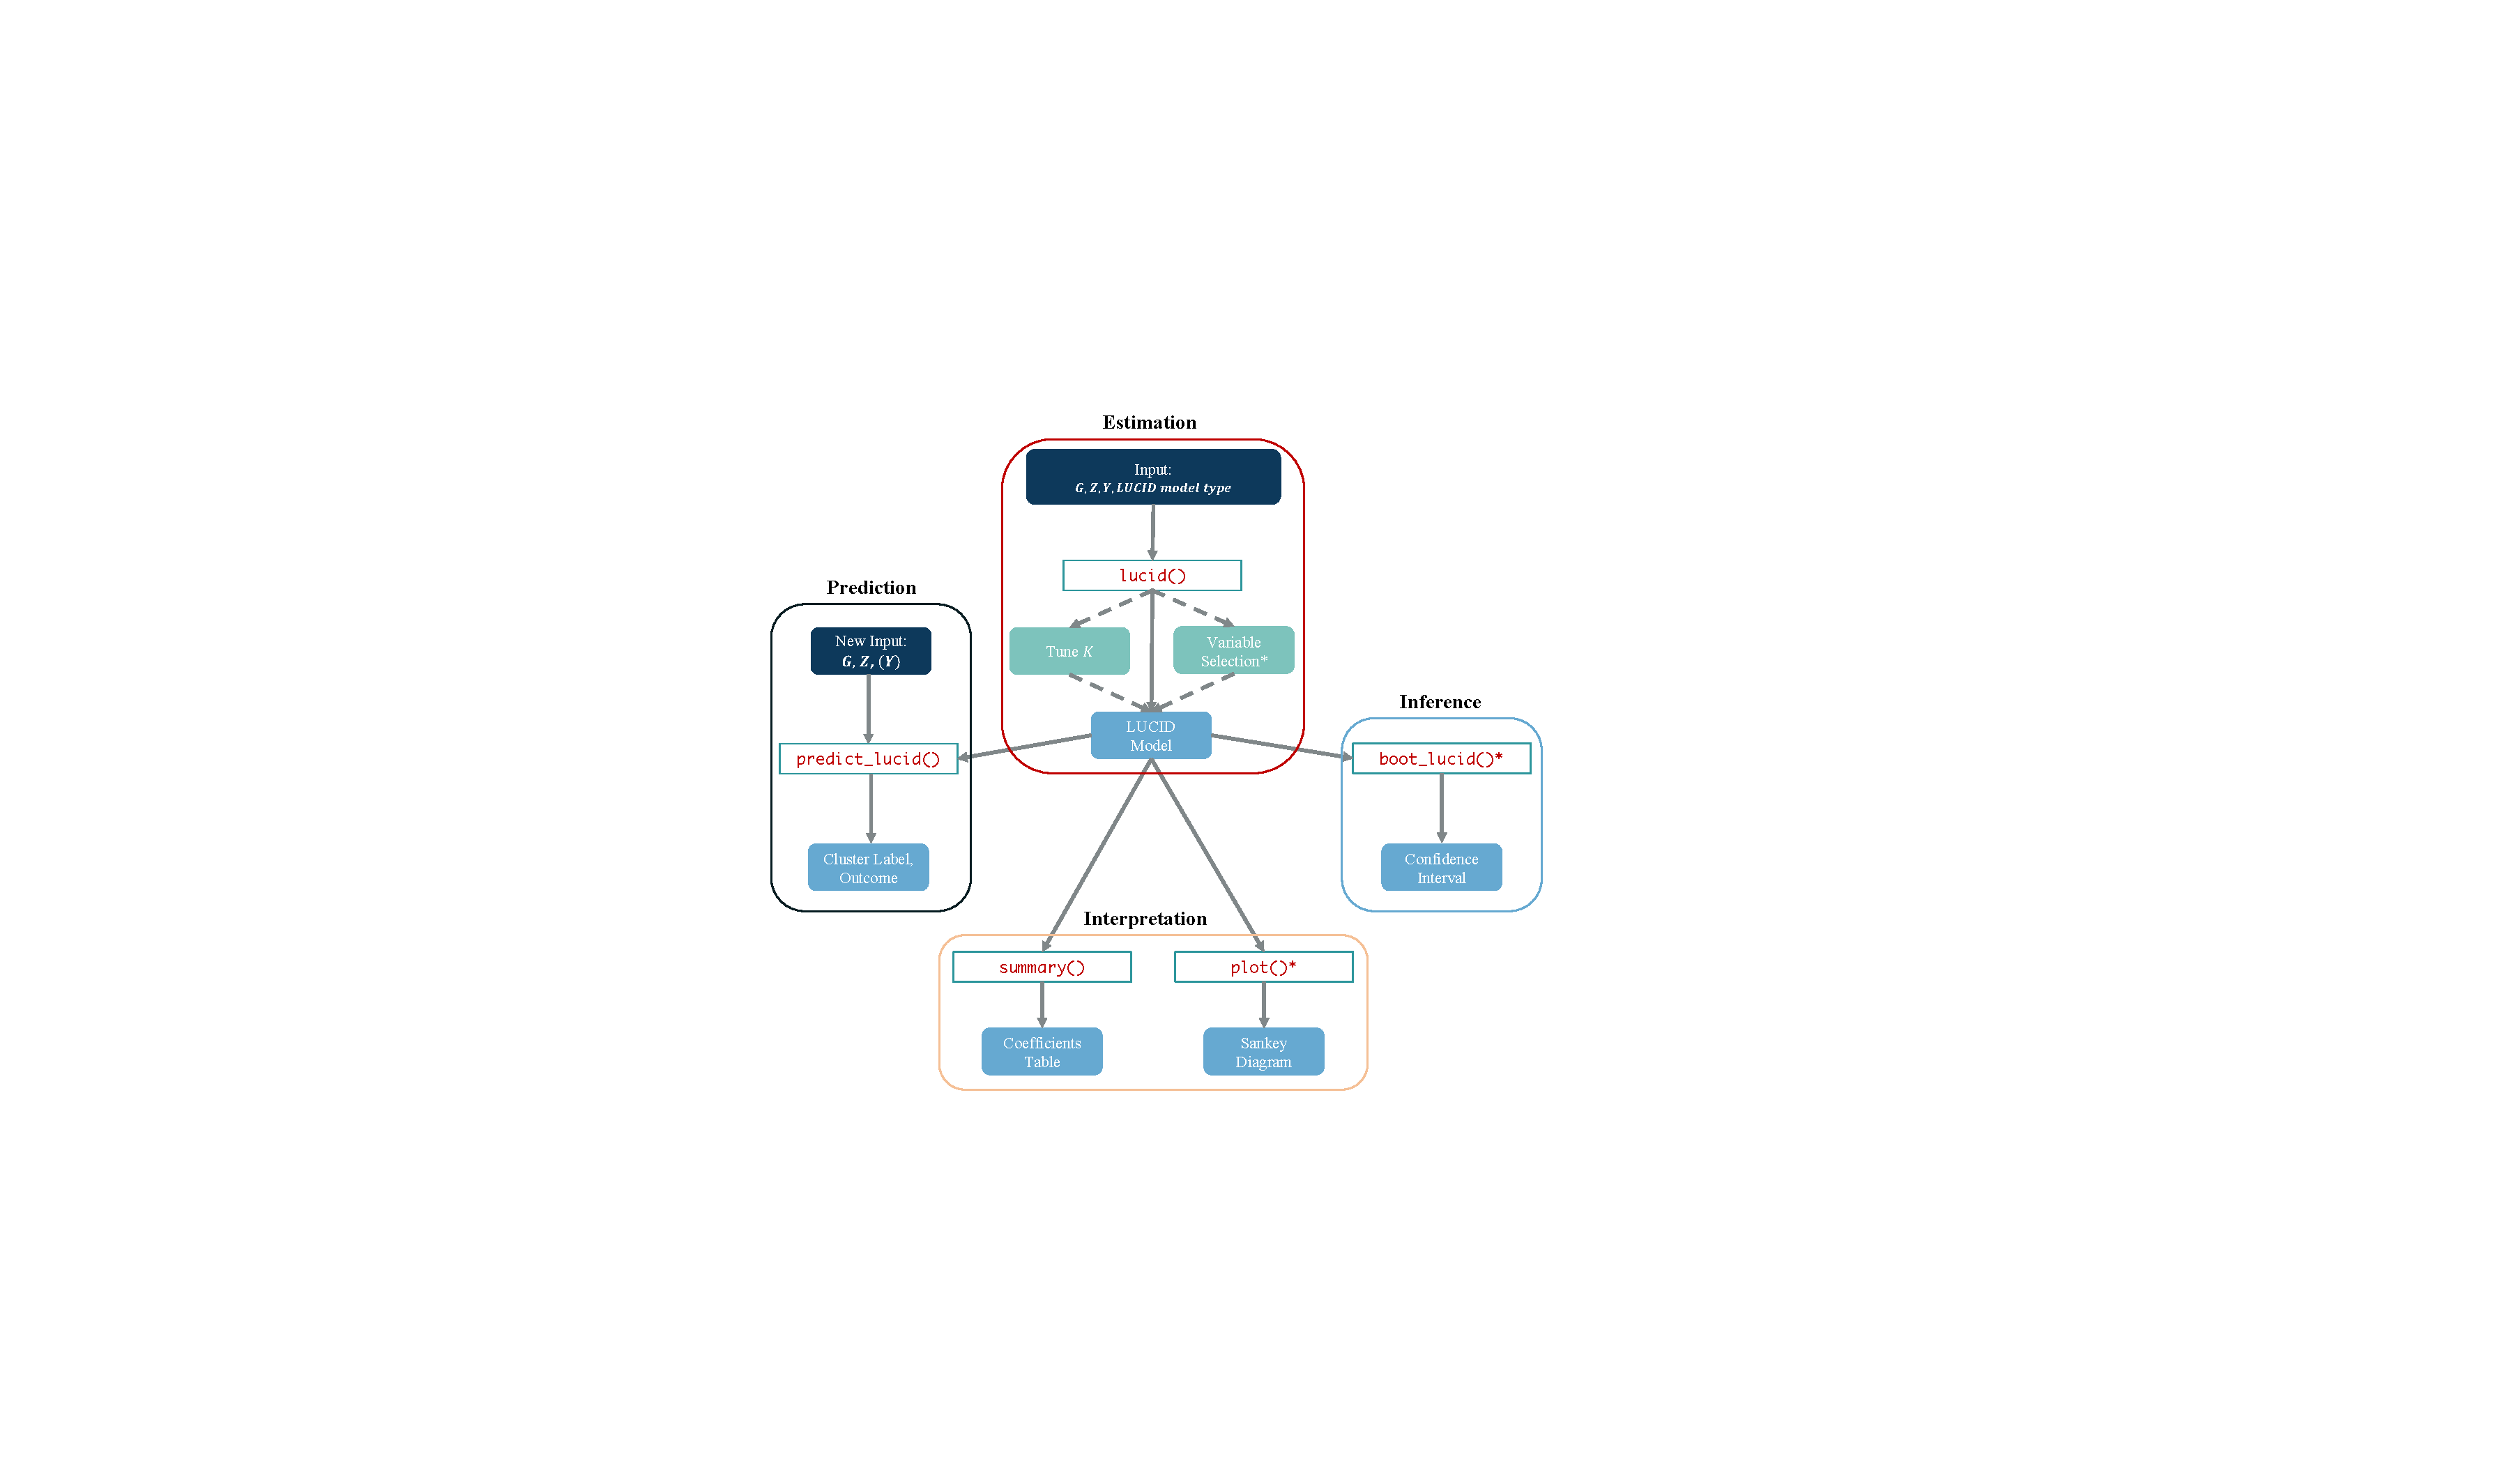
\includegraphics[scale = 0.5]{figures/fig2.pdf}
    \caption{The workflow of the \pkg{LUCIDus} package. Dark blue nodes represent input data, light blue nodes represent output results. Green nodes and dashed arrows are optional steps for model estimation. Red texts correspond to 5 key functions in \pkg{LUCIDus}. Steps and functions marked with an asterisk currently work for LUCID early integration only.}
    \label{fig2}
\end{figure}

\subsection{General workflow of \pkg{LUCIDus}} \label{sec2.2}
The \pkg{LUCIDus} package includes five main functions and two auxiliary functions to implement the analysis framework based on LUCID. Brief descriptions of each function are listed in Table \ref{tbl1}. The workflow of the \pkg{LUCIDus} package is shown in Figure \ref{fig2}. Below we describe the typical workflow of analyzing integrated data using the LUCID early integration model.
The function \code{lucid()} is the primary function in the package, which fits a LUCID model based on an exposure matrix (argument \code{G}), multi-omics data (argument \code{Z}), outcome data (argument \code{Y}), the number of latent clusters (\code{K}; default is 2), the type of the LUCID model (argument \code{lucid{\_}model}; here is \samp{early} as we focus on LUCID early integration model in this section), and the family of the outcome (argument \code{family}; default is \samp{normal}). If a vector of \code{K} and/or $L_1$ penalties are supplied, \code{lucid()} will automatically conduct model selection on the number of clusters $K$, select informative variables in $\bm G$ or $\bm Z$,  or both, and returns a LUCID early integration model (an R object of class \samp{lucid\_early}) with optimal $K$ and selected variables in $\bm G$ and/or $\bm Z$. Several additional functions can then be applied to a fitted LUCID object. \code{summary()} summarizes the fitted LUCID model by producing summary tables of parameter estimation and interpretation. Visualization is performed via the \code{plot()} function to create a Sankey diagram showing the interplay among the three components ($\bm G$, $\bm Z$, and $\bm Y$). In addition, statistical inference can be accomplished for LUCID by constructing confidence intervals (CIs) based on bootstrap resampling. This is achieved by the function \code{boot\_lucid()}. Finally, predictions on the cluster assignment and the outcome can be obtained by calling the function \code{predict\_lucid()}. In practice, it might not be necessary to implement the entire workflow above. For instance, if we have prior knowledge of the number of latent clusters $K$, model selection for the number of clusters can be skipped. If a given dataset has limited variables (for example, variables selected based on biological annotations), then variable selection may not be necessary. Note that for a LUCID in parallel model or a LUCID in serial model (the argument \code{lucid\_model} is \samp{parallel} or \samp{serial}, respectively), specification of \code{K} is different and the features of variable selection, constructing confidence intervals (CIs) based on bootstrap resampling, and plotting are not yet available (see Sections \nameref{sec_parallel} and \nameref{sec_serial}).

In the following sections, we show example code and demonstrate the usage of the LUCID early integration model using the simulated HELIX data.

%--------------------- section 3: illustration --------------------
\section{Illustration} \label{sec3}

%--------------------- section 3.1: fitting a lucid model --------------------
\subsection{Fitting a LUCID model by \code{lucid()}} \label{sec3.1}
To illustrate integrative clustering with LUCID early integration model, we use simulated data based on real cases from the HELIX study based on the correlation structure. A subset of the simulated data is incorporated in the \pkg{LUCIDus} package to replicate the workflow presented here. The dataset is a list of \code{dataframe} containing data from 420 children, with 1 variable measuring the maternal exposure to utero mercury (referred to as the exposome), 10 methylomes measured in children (referred to as the methylomics), 10 transcriptomes measured in children (referred to as the transcriptomics), 10 miRNA measured in children (referred to as the miRNA), childhood cytokeratin 18 level (referred to as ck18, a continuous outcome as an indicator of metabolic-dysfunciton-associated fatty liver disease (MAFLD), childhood cytokeratin 18 category (a binary outcome referred to as ck18{\_}cat) and 2 covariates, including child's sex and child's age. To organize the data into separate \code{dataframe}s for each type of data and to better illustrate functionality within \pkg{LUCIDus}, we use the following code: 

\begin{example}
> library(LUCIDus)
> # load data
> data("simulated_HELIX_data")
> simulated_data <- simulated_HELIX_data
> exposome <- as.matrix(simulated_data[["phenotype"]]$hs_hg_m_scaled)
> colnames(exposome) <- "hs_hg_m_scaled"
> methylomics <- simulated_data$methylome
> ck18 <- as.matrix(simulated_data[["phenotype"]]$ck18_scaled)
> colnames(ck18) <- "ck18_scaled"
> ck18_cat <- ifelse(ck18 > mean(ck18), 1, 0)
> covars <- c("hs_child_age_yrs_None","e3_sex_None")
> covs <- simulated_data[["phenotype"]][covars]
> covs$e3_sex_None <- ifelse(covs$e3_sex_None == "male", 1, 0)
\end{example}

Our goal is to conduct an integrated clustering of the exposome and methylome and to relate the estimated latent clusters to the childhood cytokeratin 18 level. The LUCID model is fitted using the function \code{lucid()}. The input data are specified by arguments \code{G}, \code{Z} and \code{Y}, corresponding to the exposome, the methylome, and the childhood cytokeratin 18 level, respectively. In practice, scaling of multi-omics data is highly recommended to obtain more stable estimates; the methylomics data used in this example are already scaled. If multi-omics data are included in the LUCID analysis as the omic intermediate $\bm Z$, the user can concatenate them one by one into a single data matrix and then input the concatenated matrix as $\bm Z$ for early integration. For illustrative purposes, we assume that, in the example data, the optimal number of latent clusters is 2 (Determining the optimal number of clusters is a major question prior to performing clustering analysis. More details are discussed in the later Section \nameref{sec3.3}). 

For illustration, we fit two LUCID models with continuous outcome ck18 and binary outcome ck18{\_}cat, respectively. The parameter \code{family} specifies the outcome type. The default setting is \samp{normal}, corresponding to a continuous outcome. For a binary outcome, \code{family} should be specified as \samp{binary}. \code{lucid()} returns an object of class \samp{lucid{\_}early} providing the MLE of the LUCID model as well as IPs.
\begin{example}
> # Fit a LUCID model with a continuous outcome
> fit1 <- lucid(G = exposome, Z = methylomics, Y = ck18, init_omic.data.model = NULL,
+               lucid_model = "early", family = "normal", K = 2)
> # MLE of the LUCID model
> # fit1$res_Beta
> # fit1$res_Mu
> # fit1$res_Sigma
> # fit1$res_Gamma
> # IPs of the sample
> # fit1$inclusion.p
> # Fit LUCID model with a binary outcome
> fit2 <- lucid(G = exposome, Z = methylomics, Y = ck18_cat, init_omic.data.model = NULL,
+               lucid_model = "early", family = "binary", K = 2)
\end{example}

%--------------------- section 3.1.1 --------------------
\subsubsection{Initializing the parameters of LUCID} \label{sec3.1.1}
$\bm \beta$ is initiated by randomly drawing from a uniform distribution. By default, \code{init\_par} is \samp{mclust} and \code{init\_omic.data.model} is \samp{EEV}, so \code{lucid()} calls \code{Mclust()} to fit the mixture model of \samp{EEV} on omics data $\bm Z$ and use the mixture model estimates to initiate $\bm \mu$ and $\bm \Sigma$, and then implement regression to initiate $\bm \gamma$. Alternatively, the user can also specify \code{init\_omic.data.model} to choose a certain mixture model. The available mixture models are listed in \code{mclust::mclustModelNames} \citep{scrucca2016mclust}. Note that \code{init\_omic.data.model} can be \samp{NULL} to let \code{Mclust()} automatically choose the optimal mixture model. If not using \code{Mclust()} for initiation, the user can also specify \code{init\_par} to be \samp{random} to initiate $\bm \mu$ and $\bm \Sigma$ by randomly drawing them from a uniform distribution and then implement regression to initiate $\bm \gamma$. We recommend using the default setting to initiate the parameters by calling \code{Mclust()} for quick convergence and stable performance.

\begin{example}
> # Fit LUCID model with spherical shape, equal volume
> fit3.1 <- lucid(G = exposome, Z = methylomics, Y = ck18, 
+                 lucid_model = "early", family = "normal", K = 2,
+                 init_par = "mclust",init_omic.data.model = "EII")
> # Fit LUCID model with random guess
> fit3.2 <- lucid(G = exposome, Z = methylomics, Y = ck18, 
+                 lucid_model = "early", family = "normal", K = 2,
+                 init_par = "random")
> # Fit LUCID model with ellipsoidal shape, varying volume, shape, and orientation 
> fit4 <- lucid(G = exposome, Z = methylomics, Y = ck18, 
+               lucid_model = "early", family = "normal", K = 2,
+               init_omic.data.model = "VVV")

\end{example}

%--------------------- section 3.1.2 --------------------
\subsubsection{Supervised LUCID versus unsupervised LUCID} \label{sec3.1.2}
In Equation \ref{eq1}, the latent clusters $\bm X$ are jointly defined by genomic/environmental exposure $\bm G$, other multi-omics data $\bm Z$, and outcome $\bm Y$. Because the outcome is explicitly incorporated in the likelihood function, the estimation process based on Equation \ref{eq1} is similar to a supervised learning process. \pkg{LUCIDus} also allows for an unsupervised version of LUCID. In this unsupervised LUCID, the latent clusters are estimated only by $\bm G$ and $\bm Z$. Specifically, the joint likelihood of unsupervised LUCID is written as
\begin{equation}
    \begin{aligned}
         \log L(\bm{\Theta}) & = \sum_{i = 1}^N \sum_{j=1}^K I(X_i = j) \left( \log S(X_i = j| \bm{G}_i; \bm{\Theta}) + \log \phi(\bm{Z}_i| X_i = j; \bm{\Theta})\right)
    \end{aligned}
    \label{eq11}
\end{equation}
and the corresponding responsibility based on Equation \ref{eq11} is derived as
\begin{equation}
    \begin{aligned}
        r_{ij}^{(t)} & = \frac{S\left(X_i = j| \bm{G}_i; \bm{\beta}^{(t)}\right) \phi\left(\bm{Z}_i| X_i = j; \bm{\mu}_j^{(t)}, \bm{\Sigma}_j^{(t)}\right)}{\sum_{j = 1}^K S\left(X_i = j| \bm{G}_i; \bm{\beta}^{(t)}\right) \phi\left(\bm{Z}_i| X_i = j; \bm{\mu}_j^{(t)}, \bm{\Sigma}_j^{(t)}\right)}
    \end{aligned}
    \label{eq12}
\end{equation}
Estimations for unsupervised LUCID are also obtained by the EM algorithm discussed previously. The parameter \code{useY} in \code{lucid()} is a flag indicating a supervised or unsupervised LUCID model. By default, \code{useY = TRUE} and \code{lucid()} fit supervised LUCID. To fit an unsupervised LUCID model, a user should set \code{useY = FALSE}.
\begin{example}
> # Fit an unsupervised LUCID model
> fit5 <- lucid(G = exposome, Z = methylomics, Y = ck18, lucid_model = "early", 
+               family = "normal", K = 2, useY = FALSE)
\end{example}
The choice of a supervised LUCID or unsupervised LUCID model depends both on the study design and the research question. A supervised LUCID analysis may be appropriate, for example, if: (1) there is the belief that the cluster structure is defined jointly by $\bm G$, $\bm Z$ and $\bm Y$ (for example, data collected from a cross-sectional design); or (2) the goal is to build a predictive model with data from one cohort to then apply directly to another cohort. If the aim is to obtain an unbiased estimate for the association between the latent cluster $\bm X$ and the outcome $\bm Y$, an unsupervised LUCID model is more appropriate. 

%--------------------- section 3.1.3: adjusting for covariates --------------------
\subsubsection{Adjusting for covariates} \label{sec3.1.3}
\pkg{LUCIDus} also allows for the adjustment of covariates. According to the DAG in Figure \ref{fig1} (a), covariates may be included for the association between the exposure and the latent cluster (referred to as $\bm G$ to $\bm X$ covariate) or for the association between the latent cluster and the outcome (referred to as $\bm X$ to $\bm Y$ covariate). Covariates in the $\bm G$ to $\bm X$ relationship act more like predictors of the latent cluster while covariates in the $\bm X$ to $\bm Y$ relationship may be interpreted more in the context of an adjustment for a potential confounding effect. A variable can serve as both a $\bm G$ to $\bm X$ covariate and a $\bm X$ to $\bm Y$ covariate. In the \code{lucid()} function, $\bm G$ to $\bm X$ covariates are specified by parameter \code{CoG} and $\bm X$ to $\bm Y$ covariates are specified by parameter \code{CoY}.
\begin{example}
> # Include covariates as G to X covariates
> fit6 <- lucid(G = exposome, Z = methylomics, Y = ck18, lucid_model = "early", K = 2, 
+               family = "normal", CoG = covs)
> # Include covariates as X to Y covariates
> fit7 <- lucid(G = exposome, Z = methylomics, Y = ck18, lucid_model = "early", K = 2, 
+               family = "normal", CoY = covs)
\end{example}




%--------------------- section 3.2: interpreting LUCID --------------------
\subsection{Interpreting LUCID} \label{section3.2}
Since LUCID is an integrated analysis framework consisting of clustering, regression, and multiple data components, we provide two utility functions, \code{summary()} and \code{plot()} to summarize the results of LUCID and to facilitate interpretation.

%--------------------- section 3.2.1: visualization --------------------
\subsubsection{Summarizing LUCID in tables by \code{summary()}}
 A direct call of \code{summary()} with the input of a model returned by \code{lucid()} prints three tables in the console, corresponding to associations among $\bm G$, $\bm Z$ and $\bm Y$. We take the LUCID model fitted with the continuous BMI as an example.
\begin{example}
> # summarize a simple lucid model with a continuous outcome
> summary(fit1)
----------Summary of the LUCID Early Integration model---------- 
 
K =  2 , log likelihood = -6721.801 , BIC =  14808.7 
 
(1) Y (continuous outcome): effect size of Y for each latent cluster
             Gamma
cluster1 0.0000000
cluster2 0.5040367

(2) Z: mean of omics data for each latent cluster 
              mu_cluster1 mu_cluster2
cg_GRHL3        0.2452019  -0.3627827
cg_BTF3L4       0.1863510  -0.2798288
cg_AL358472.7   0.1954543  -0.3290283
cg_HDGF         0.1897587  -0.2614602
cg_TDRD5        0.1977435  -0.2186209
cg_CSRNP3       0.1742812  -0.1794667
cg_HSPD1        0.2829609  -0.3282916
cg_EPM2AIP1    -0.1565522   0.3031461
cg_AC025171.1   0.2769363  -0.2656729
cg_VTRNA1_3    -0.2250234   0.1847493

(3) E: odds ratio of being assigned to each latent cluster for each exposure 
                             beta       OR
hs_hg_m_scaled.cluster2 0.7909168 2.205417
\end{example}
The first table summarizes the association between the latent cluster and the outcome (cytokeratin 18). The estimated effect size of cytokeratin 18 for cluster 1 is 0 since it is the reference cluster while that for cluster 2 is 0.504. In the case of binary outcome, the coefficient in the first table is interpreted as the log odds for the variable for that specific cluster vs. the reference cluster. The second table characterizes each cluster by its omics signature. The omics signature is a cluster-specific mean for each variable in the omics data. For instance, latent cluster 1 is characterized by low levels of cg{\_}EPM2AIP1 ($\mu_1 (\text{cg{\_}EPM2AIP1})= -0.157$) and cg{\_}VTRNA1{\_}3 ($\mu_1 (\text{cg{\_}VTRNA1{\_}3})= -0.225$), and high levels of all other omic features, for example, cg{\_}GRHL3 ($\mu_1 (\text{cg{\_}GRHL3})= 0.2452019$). On the contrary, latent cluster 2 features high levels of cg{\_}EPM2AIP1 ($\mu_2 (\text{cg{\_}EPM2AIP1})=  0.303$) and cg{\_}VTRNA1{\_}3 ($\mu_2 (\text{cg{\_}VTRNA1{\_}3})= 0.185$), and low levels of all other features including cg{\_}GRHL3 ($\mu_2 (\text{cg{\_}GRHL3})= -0.363$). The third table relates the exposures to the latent clusters. For instance, \samp{hs{\_}hg{\_}m{\_}scaled} represents the scaled level of maternal mercury exposure. The coefficient OR for \samp{hs{\_}hg{\_}m{\_}scaled} is 0.791, meaning for each doubling of the scaled level of maternal mercury exposure, the odds ratio of being assigned to latent cluster 2 is 2.205. Since latent cluster 2 is associated with a higher child level of cytokeratin 18, these results indicate that exposure to mercury is associated with a higher child level of cytokeratin 18 and thus higher risks of MAFLD.

%--------------------- section 3.2.2 --------------------
\begin{figure}[]
    \centering
    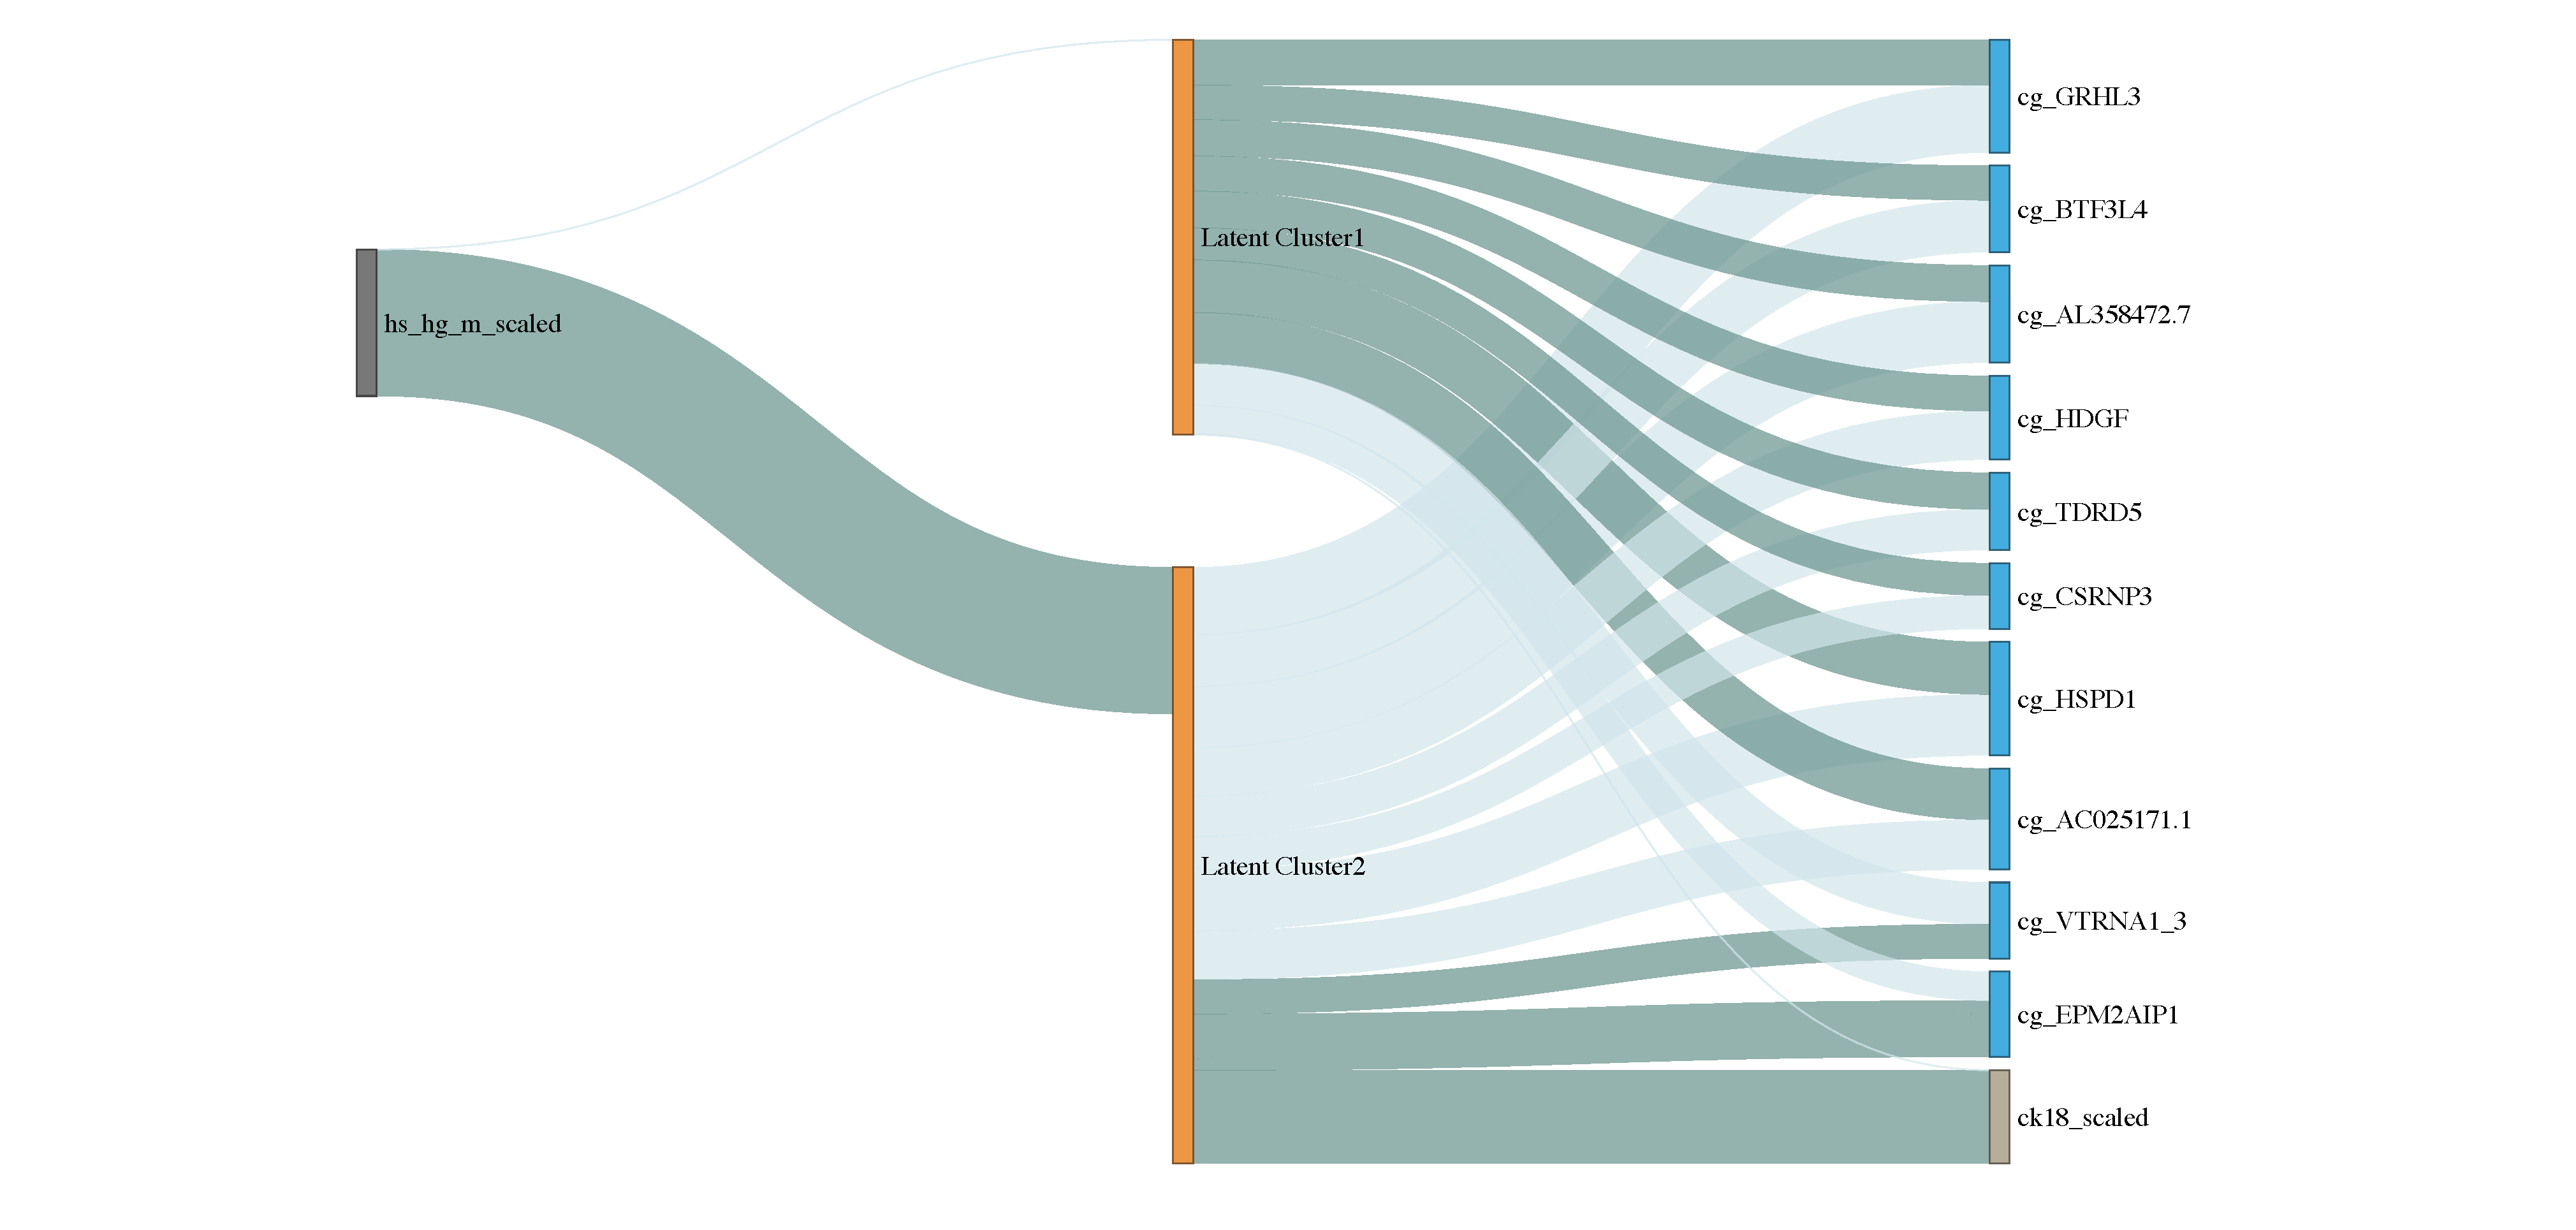
\includegraphics[width = \textwidth]{figures/fig3.pdf}
    \caption{An example of using the Sankey diagram to visualize a LUCID model. The dark grey nodes represent the exposure, the light grey node represents the outcome, the blue nodes are omics data and the orange nodes are latent clusters. The width of links and nodes corresponds to effect size. Light-colored links represent negative associations while dark-colored links indicate positive associations.}
    \label{fig3}
\end{figure}
\subsubsection{Visualizing LUCID by \code{plot()}} \label{sec3.2.2}
Visualization is another imperative way to interpret statistical models. Here we use a Sankey diagram \citep{schmidt2008sankey} for visualization of the relationships among different components in LUCID. \code{plot()} takes a fitted LUCID model as input and creates a Sankey diagram in \code{html} format. It also accepts a user-defined color palette. 
\begin{example}
> # Visualize LUCID model via a Sankey diagram
> plot(fit1)
> # Change the node color
> plot(fit1, G_color = "yellow")
> # Change the link color
> plot(fit1, pos_link_color = "red", neg_link_color = "green")
\end{example}
Figure \ref{fig3} shows an example of a Sankey diagram for the example data. Each node represents a component in the LUCID model. Different components are labeled by user-defined colors. Each link represents the statistical association between two nodes. The width of the links reflects the effect size of the association, and the color of the links indicates the direction of the  association. By default, dark-colored links represent positive associations while light-colored links indicate negative associations. The output of the Sankey diagram is an interactive html file in which the user can drag and re-arrange the layout of the elements, to avoid overlapping. In practice, we recommend limiting the number of variables in the Sankey diagram to ~10 to facilitate interpretation.

%--------------------- section 3.3--------------------
\begin{figure}[]
    \centering
    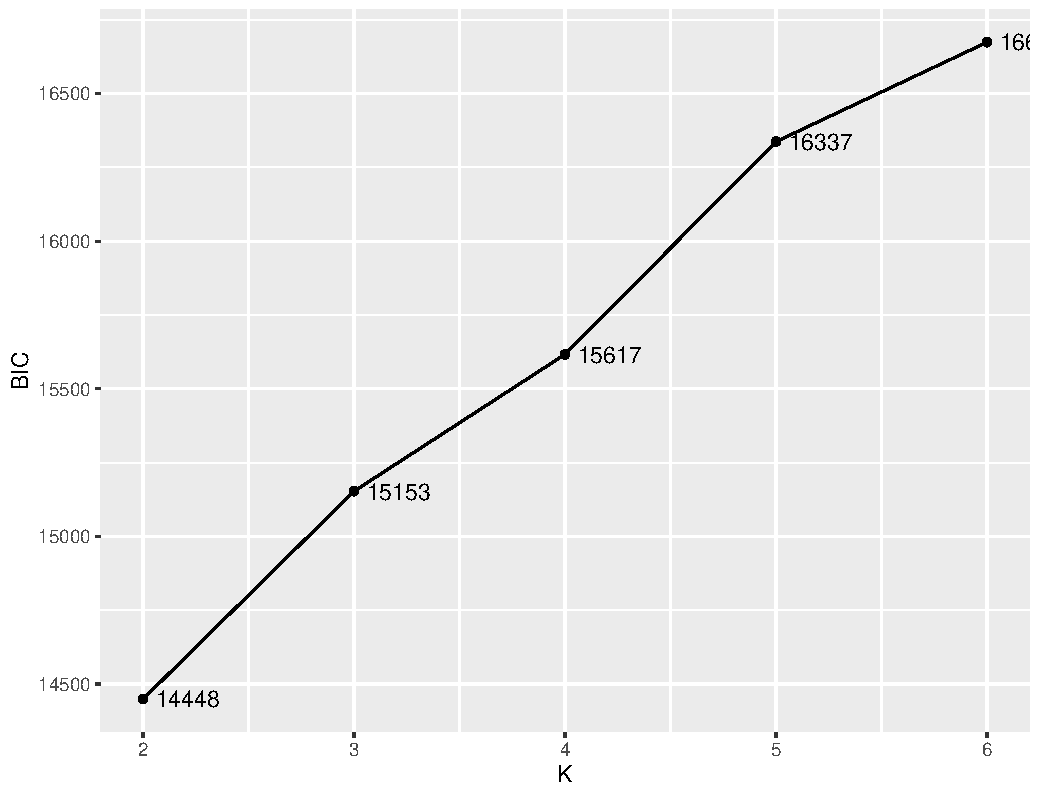
\includegraphics[scale = 0.6]{figures/fig4.pdf}
    \caption{Choosing optimal number of latent clusters K based on BIC.}
    \label{fig4}
\end{figure}
\subsection{Model selection and variable selection} \label{sec3.3}
To determine the number of latent clusters, $K$, LUCID implements model selection by fitting a series of models, each with a different value for $K$, and then the Bayesian Information Criteria (BIC) is used to choose the optimal model \citep{fan2013tuning}. The optimal model is the one with the lowest BIC. The BIC for LUCID is defined as
\begin{equation}
    \text{BIC} = -2 \log L(\hat{\bm \Theta}) + D \log N
\end{equation}
where $\hat{\bm \Theta}$ is the maximum likelihood estimation and $D$ is the number of parameters in LUCID. Specifically, $D = P(K - 1) + KM + KM(M + 1)/2 + n_Y$, where $n_Y$ is the number of parameters dependent upon the type of outcome $\bm Y$. If $\bm Y$ is a continuous outcome, then $n_Y = 2K$. If $\bm Y$ is a binary outcome, then $n_Y = K$. If a vector of $K$ is used as input to the function \code{lucid()}, model selection is automatically performed and returns the model with optimal $K$.
\begin{example}
> fit8 <- lucid(G = exposome, Z = methylomics, Y = ck18, lucid_model = "early", 
+               family = "normal", K = 2:6)
> # Check the optimal K
> fit8$K
[1] 2
\end{example}

Separately, users can use the auxiliary function \code{tune\_lucid()} to look into model selection in more details. This function returns the optimal model as well as a table recording the tuning process. Below is an example of tuning $K$ and visualizing the tuning process by using \code{tune\_lucid()}.
\begin{example}
> # Look into the tuning process in more details
> tune_K <- tune_lucid(G = exposome, Z = methylomics, Y = ck18, lucid_model = "early", 
+                      family = "normal", K = 2:6)
> fit9 <- tune_K$best_model
> ggplot(data = tune_K$tune_list, aes(x = K, y = BIC, label = round(BIC, 0))) + 
+   geom_point() +
+   geom_line() + 
+   geom_text(hjust = -0.2)
\end{example}
Figure \ref{fig4} shows the tuning process with $K = 2$ resulting in the lowest BIC.

Including additional or redundant variables in clustering models may increase model complexity, impair prediction accuracy, and boost computational time \citep{fop2018variable}. \pkg{LUCIDus} performs variable selection for both the genetic/environmental exposures $\bm G$ and for the other multi-omics data $\bm Z$ via $L_1$-norm penalty terms. For variable selection for $\bm G$, we apply the LASSO regression to obtain sparse solutions for Equation \ref{eq5}, which is
\begin{equation}
     \bm{\beta}_{\text{LASSO}}^{(t+1)} = \arg \max_{\bm{\beta}} \left\{ \sum_{i = 1}^N \sum_{j = 1}^K r_{ij}^{(t)}\log S(X_i = j | \bm{G}_i; \bm{\beta}_j) - \lambda_{\bm{\beta}}\sum_{j = 1}^K\sum_{l = 1}^P |\beta_{jl}| \right\}
     \label{eq14}
\end{equation}
To obtain sparse estimation for $\bm \mu$ and $\bm \Sigma$, we implement the penalized model-based method \citep{zhou2009penalized}. $\bm \mu$ is first updated by maximizing the following equation,
\begin{equation}
    \bm{\mu}_j^{(t+1)} = \arg \max_{\bm \mu} \left \{ \sum_{i = 1}^N \sum_{j = 1}^K r_{ij}^{(t)}\log \phi(\bm{Z}_i| \bm{\mu_j}, \bm{\Sigma_j}) - \lambda_{\bm{\mu}}\sum_{j = 1}^K\sum_{l = 1}^M |\mu_{jl}| \right \}
    \label{eq15}
\end{equation}
Denote $\bm{W} = \bm{\Sigma}^{-1}$. Then $\bm \Sigma$ is updated by maximizing its inverse penalized by $L_1$-norm
\begin{equation}
    \bm{W}_j^{(t+1)} = \arg \max_{\bm W} \left \{ \sum_{i = 1}^N \sum_{j = 1}^K r_{ij}^{(t)}\left( \det \bm{W}_j - \text{trace}(\bm{S}_j^{(t)} \bm{W}_j) \right) - \lambda_{\bm{W}}\sum_{ls}|w_{jls}| \right \}
    \label{eq16}
\end{equation}
where $\bm S_j$ is the empirical covariance matrix at each iteration, defined as 
\begin{equation}
    \bm{S}_j^{(t)} = \frac{\sum_{i=1}^N r_{ij}\left(\bm{Z}_i - \bm{\mu}_j^{(t)}\right)\left(\bm{Z}_i - \bm{\mu}_j^{(t)}\right)^T}{\sum_{i=1}^N r_{ij}^{(t)}}
    \label{eq17}
\end{equation}

To choose the optimal combination of the three $L_1$-norm penalties, we implement a grid-search by adopting a modified BIC \citep{pan2007penalized}, defined as 
\begin{equation}
    \text{BIC}_p = -2 \log L(\hat{\bm \Theta}) + (D - D_{\bm G} - D_{\bm Z})\log N
    \label{eq18}
\end{equation}
Where $D_{\bm G}$ is the number of exposure variables whose effect estimates are 0 across all latent clusters and $D_{\bm Z}$ is the number of omic variables whose effect estimates are 0 across all latent clusters. We can tune $\lambda_{\bm \beta}$, $\lambda_{\bm \mu}$ and $\lambda_{\bm W}$ either separately or jointly. For instance, if only exposome data $\bm G$ is high-dimensional, we only need to tune $\bm \lambda_{\bm \beta}$. If variable selection is desired for both $\bm G$ and $\bm Z$, then the three $L_1$-norm penalties should be tuned simultaneously. $\lambda_{\bm \beta}$, $\lambda_{\bm \mu}$ and $\lambda_{\bm W}$ match the parameters \code{Rho\_G}, \code{Rho\_Z\_Mu} and \code{Rho\_Z\_Cov} in the \code{lucid()} function. Each parameter accepts a numeric vector or a scalar as input. For guidance, empirical experiments utilizing normalized multi-omics data suggest integer values in the range of $0 - 100$ for \code{Rho\_Z\_Mu} and values in the range of $0 - 1$ for \code{Rho\_G} and \code{Rho\_Z\_Cov}. The higher the values of \code{Rho\_Z\_Mu}, \code{Rho\_G}, and \code{Rho\_Z\_Cov}, the fewer omic features that will be selected. Below are examples for conducting variable selection in $\bm G$ and $\bm Z$, separately and jointly.
\begin{example}
> # Variable selection for G
> # Add 10 more noise variables to the exposome
> noise <- matrix(rnorm(420 * 10), nrow = 420)
> exposome_noise <- cbind(exposome, noise)
>  fit10 <- lucid(G = exposome_noise, Z = methylomics, Y = ck18, 
+                 lucid_model = "early", family = "normal", K = 2,
+                 Rho_G = seq(0, 0.4, by = 0.01), seed = 1008)

1/11 exposures are selected

> # Summary of optimal lucid model
> # summary(fit10)
> 
> # Variable selection for Z
> # add 10 more noise variables to the methylomics
> methylomics_noise <- cbind(methylomics, noise)
> fit11 <- lucid(G = exposome, Z = methylomics_noise, Y = ck18, 
+                lucid_model = "early", family = "normal", K = 2,
+                Rho_Z_Mu = 5:10, Rho_Z_Cov = seq(0.1, 0.4, by = 0.1), seed = 1008)

10/20 omics variables are selected  

> # Summary of optimal lucid model
> # summary(fit11)
> 
> # Variable selection for G and Z jointly
> fit12 <- lucid(G = exposome_noise, Z = methylomics_noise, Y = ck18, 
+                lucid_model = "early", family = "normal", K = 2,
+                Rho_G = 0.01, Rho_Z_Mu = 10, Rho_Z_Cov = 0.5, seed = 123)

1/11 exposures are selected 
11/20 omics variables are selected 
\end{example}

Oftentimes, the number of features $M$ for omics data $\bm Z$ is in the hundreds or even thousands. With a high dimensionality of $\bm Z$, LUCID can still have a stable performance and select the features with effect if the number of observations $N$ is higher than $M$. Below is an example of conducting variable selection in $\bm Z$ with $M$ = 210 features (including 200 noise features) while $N$ = 420. We can see that with higher \code{Rho\_Z\_Mu} and \code{Rho\_Z\_Cov}, LUCID successfully selects the features with effect. 

\begin{example}
> # Variable selection for Z (high number of features M)
> set.seed(1008)
> # Add 200 more noise features to the methylomics
> noise <- matrix(rnorm(420 * 200), nrow = 420)
>  methylomics_noise <- cbind(methylomics, noise)
> fit13 <- lucid(G = exposome, Z = methylomics_noise, Y = ck18, 
+                family = "normal", lucid_model = "early", K = 2,
+                Rho_Z_Mu = 20, Rho_Z_Cov = 0.6)

17/210 omics variables are selected 

> # Summary of optimal lucid model
> # summary(fit13)
\end{example}

Via simulations running time for LUCIDus increases linearly as the number of features increases. While the integration of regularization allows for a high number of features to be analyzed, when $M$ is higher than $N$, LUCID might result in unstable estimation, therefore pre-screening approaches for the omic features such as the "meet-in-the-middle" become imperative to reduce dimensionality before fitting the LUCID model \citep{CADIOU2021106509}.

%--------------------- section 3.4 --------------------
\subsection{Deriving confidence intervals} \label{sec3.4}
We use the nonparametric bootstrap approach to derive confidence intervals (CIs) for the MLE estimates from a LUCID model \citep{davison1997bootstrap}. Nonparametric bootstrap draws observations from a sample with replacement. We index the bootstrap samples by $b = 1, 2, \ldots, B$. For each bootstrap sample $\bm{D}^b$, we fit the LUCID model and calculate MLE $\bm{\Theta}^b$. Two types of bootstrap CIs are constructed based on the distribution of $\bm{\Theta}^b$: (1) normal CIs and (2) percentile CIs.

Given the confidence level $1 - \alpha$, the normal CIs are constructed by 
\begin{equation}
    (1 - \alpha)\% \text{CI}_{\text{normal}} = \bm{\Theta} - \text{bias} \pm Z_{1 - \alpha/2}\sigma(\bm \Theta)
    \label{eq19}
\end{equation}
where $\text{bias} = \bar{\bm \Theta} - \bm{\Theta}$, $\bar{\bm \Theta}$ is the mean of the bootstrap estimators and $\sigma(\bm \Theta)$ is the bootstrap standard error, which is
\begin{equation}
    \sigma(\bm \Theta) = \sqrt{\frac{1}{B - 1}\sum_{b=1}^B\left(\bm{\Theta}^b - \bar{\bm \Theta}\right)}
    \label{eq20}
\end{equation}
All calculations in Equation \ref{eq19} and \ref{eq20} are elementwise.

In addition, the $1 - \alpha$ percentile CIs are calculated by ordering the bootstrap estimators from smallest to largest and selecting the estimates at $\alpha/2$ percentile and $(1 - \alpha/2)$ percentile as the CIs.

\code{boot\_lucid()} constructs the two bootstrap CIs described above for inference. Users can specify the confidence level (\code{conf}) and the number of bootstrap replicates (\code{R}). While \code{boot\_lucid()} is running, a progress bar is displayed in the R console. We recommend \code{R} $\geq 200$ to estimate the bootstrap standard error for normal CIs and \code{R} $\geq 800$ to estimate quantiles to construct percentile CIs. Below are examples of deriving bootstrap CIs for LUCID. By default, LUCID calculates $95\%$ CIs.
\begin{example}
> # Bootstrap to obtain 95% CI (by default) for LUCID
> set.seed(123)
> boot1 <- boot_lucid(G = exposome, Z = methylomics, Y = ck18, lucid_model = "early", 
+                     model = fit1, R = 200)
# 90% CIs
> boot2 <- boot_lucid(G = exposome, Z = methylomics, Y = ck18, lucid_model = "early", 
+                     model = fit1, R = 200, conf = 0.9)
\end{example}

We can obtain a more comprehensive summary table with bootstrap CIs by integrating \code{summary()} with output from \code{boot\_lucid()}. The resulting summary table has 5 columns: \samp{t0} corresponds to parameters estimated from the observed data; \samp{norm\_lower} and \samp{norm\_upper} represent the lower and upper limit of normal CIs, respectively; \samp{perc\_lower} and \samp{perc\_upper} represents the percentile CIs.
\begin{example}
> # Summary table with 95% bootstrap CIs
> summary(fit1, boot.se = boot1))
\end{example}

\code{boot\_lucid()} is built upon the R library \CRANpkg{boot} \citep{canty2021boot}. The original output from \pkg{boot} is also returned by \code{boot\_lucid()} and can be used to evaluate the normality of the distribution of the bootstrap estimations.

%--------------------- section 3.5: prediction --------------------
\subsection{Prediction}
The prediction of LUCID includes two parts: prediction of the latent clusters $\bm X$ and prediction of the outcome $\bm Y$. The \code{predict\_lucid()} can perform both tasks. Prediction for latent cluster is determined by IP using the optimal rule, which is
\begin{equation}
    \hat{X}_i = \arg \max_j P(X_i = j| \bm{D}, \bm{\Theta})
    \label{eq21}
\end{equation}

Prediction for outcome follows a conventional regression framework. When making predictions, \code{predict\_lucid()} for LUCID requires an input of a new $\bm G$ and $\bm Z$, and optional input of $\bm Y$. If $\bm Y$ is provided, we use Equation \ref{eq3} to calculate IPs; otherwise, Equation \ref{eq12} is applied. As a result, we can either fit a supervised LUCID model to make predictions in an unsupervised fashion or vice versa. This design allows for flexibility. For instance, we can build a LUCID model in one cohort in a supervised fashion, and then make predictions on another new independent cohort, regardless of whether the outcome is measured or not. \code{predict\_lucid()} for LUCID returns a \code{list} containing IPs for each observation, predicted cluster assignment, and predicted outcome. Below is an example code for prediction based on a supervised LUCID model, \code{fit1}.
\begin{example}
> # Predict cluster with information of Y
> pred1 <- predict_lucid(model = fit1, G = exposome, Z = methylomics, Y = ck18)
> # Predict cluster without information of Y
> pred2 <- predict_lucid(model = fit1, G = exposome, Z = methylomics)
> # Predicted cluster label
> table(pred1$pred.x)

  1   2 
223 197 
> # Predicted outcome
> pred1$pred.y[1:5]
[1]  0.2580164 -0.3806054  0.2504817  0.4123169 -0.1898255
\end{example}

%--------------------- section 3.6 --------------------
\begin{figure}
    \centering
    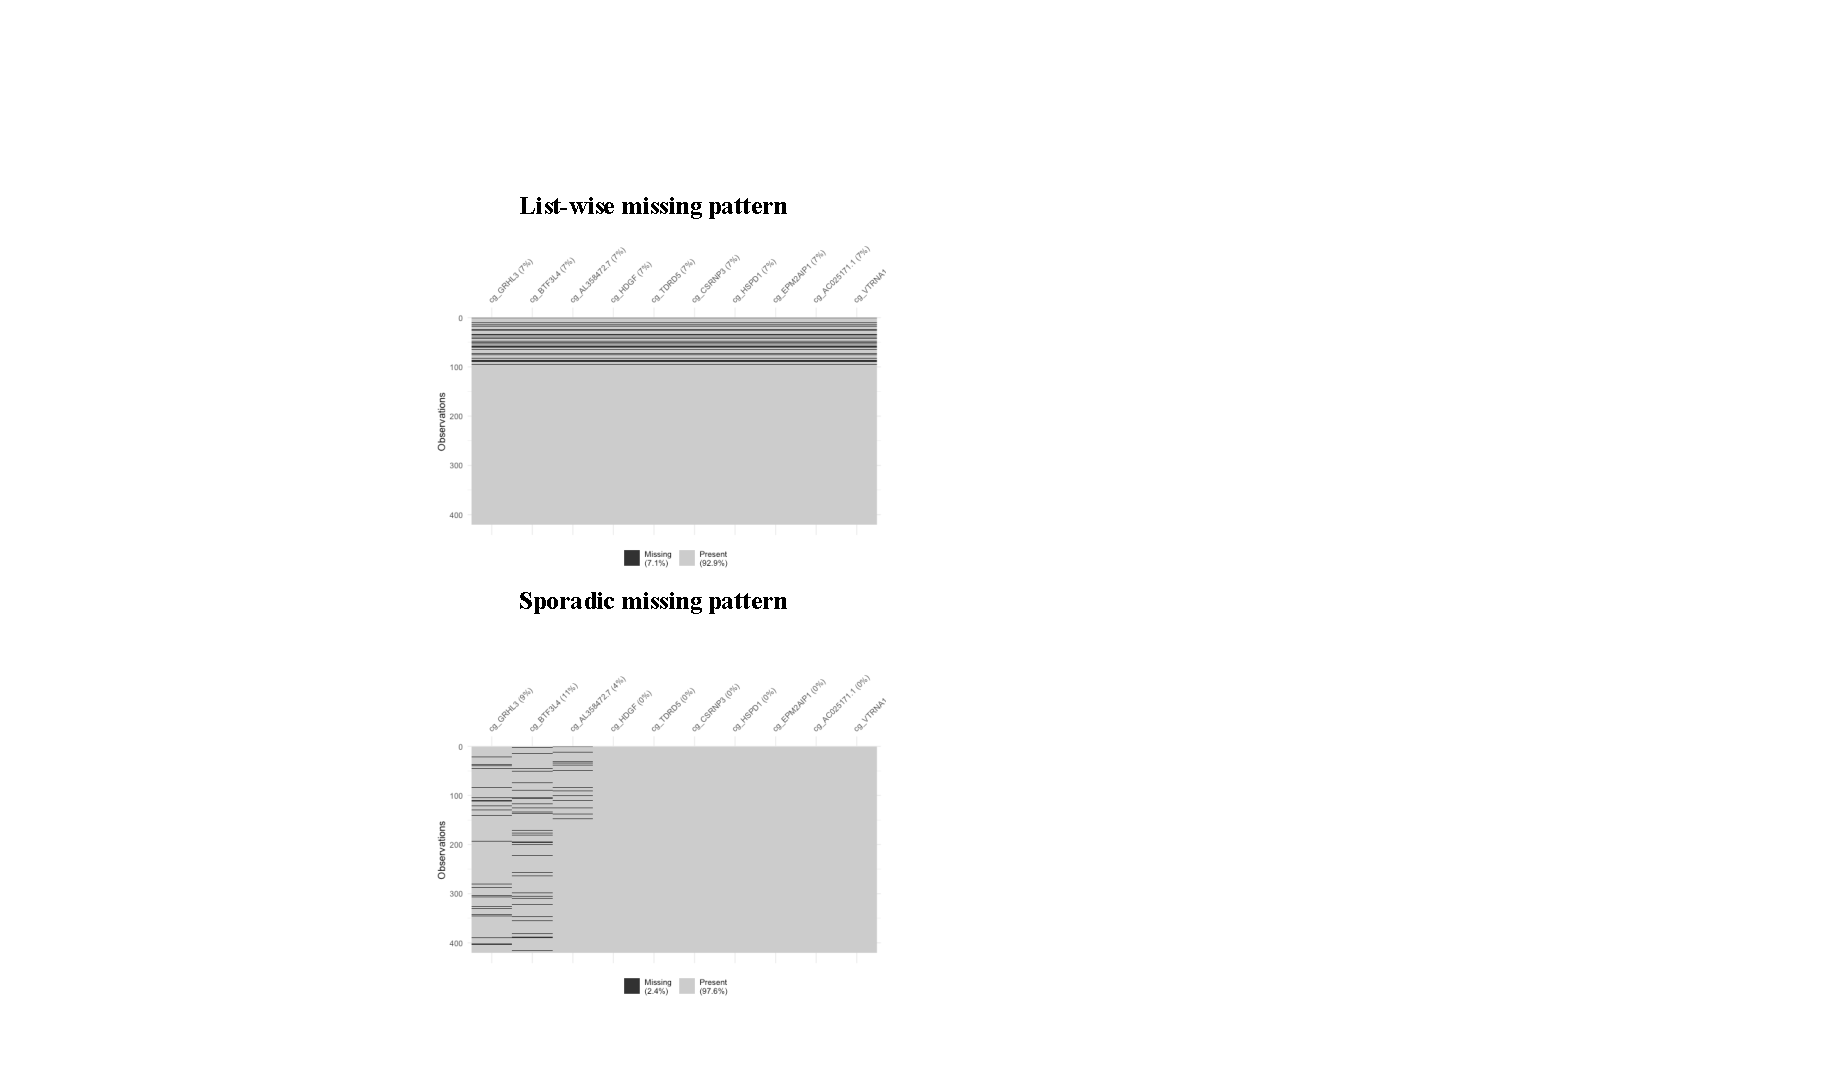
\includegraphics[scale = 1.2]{figures/fig5.pdf}
    \caption{Two simulated missing patterns in methylomics data}
    \label{fig5}
\end{figure}

\subsection{Incorporating missingness in multi-omics data}
A major update in \pkg{LUCIDus} version 3 is the incorporation of missing data. Missingness is a major challenge in the integrative analysis of omics. In large cohort studies, it is common that some omics data are not available for all participants for various reasons such as budgetary constraints, low sample availability, or lack of consent for future use of biospecimens \citep{voillet2016handling}. We refer to this type of missingness as a list-wise missingness pattern. In addition, even when omics data are measured for a given participant, it is common that some omic features are randomly missing due to the measurement process. We refer to this pattern as sporadic missingness. \pkg{LUCIDus} can deal with the two missing patterns mentioned above or the combination of the two. We assume the multi-omics data are missing completely at random (MCAR) for both missing patterns(i.e. for list-wise missing pattern, the probability of multi-omics data being not available is the same for all subjects; for sporadic missing pattern, the probability of a certain omic feature being missing is the same for all omic features). 

For list-wise missingness, we use a modified LUCID model based on a likelihood partition. We divide the LUCID likelihood into two parts: observations with complete multi-omics data and observations without any measured multi-omics data. The likelihood of the former observations remains the same as Equation \ref{eq2}, denoted by $l_o (\bm{\Theta}|\bm{D})$. The joint likelihood of the latter observations becomes
\begin{equation}
    l_m(\bm{\Theta}|\bm{D}) = \sum_{l_o=1}^{N_o}\sum_{j=1}^K I(X_{i_o} = j) \left( \log S(X_{i_o} = j| \bm{G}_{i_o};\bm{\beta}_j) + \log \phi\left(Y_{i_o}|\gamma_j, \sigma_j^2\right)\right)
    \label{eq22}
\end{equation}
with corresponding responsibility defined as 
\begin{equation}
    \begin{aligned}
        r_{ij}^{(t)} = \frac{S\left(X_i = j| \bm{G}_i; \bm{\beta}^{(t)}\right) \phi\left(Y_i|X_i = j; \gamma_j^{(t)}, \sigma^{2(t)}_j \right)}{\sum_{j = 1}^K S\left(X_i = j| \bm{G}_i; \bm{\beta}^{(t)}\right) \phi \left(Y_i|X_i = j; \gamma_j^{(t)}, \sigma^{2(t)}_j\right)}
    \end{aligned}
    \label{eq23}
\end{equation}
The joint likelihood of LUCID for all data becomes $l(\bm{\Theta}) = l_o (\bm{\Theta}|\bm{D}) +l_m (\bm{\Theta}|\bm{D})$. We then use the same EM algorithm described in Section \nameref{sec2.1} to calculate the MLE of LUCID with list-wise missingness.

For sporadic missingness, we use an integrated imputation method \citep{zhang2021gaussian}. Each missing value in the omics data $\bm Z$ is treated as an unknown ``parameter'' to be optimized. Specifically in the M-step, after maximizing the parameters of LUCID model with fixed $\bm Z$, we implement an additional \emph{imputation step} which maximizes $\bm Z$ with fixed parameters within LUCID. Details of the statistical derivation can be found in \citet{zhang2021gaussian}.

To illustrate this new feature, we first simulate missing values in the HELIX methylomics data by randomly setting values to \samp{NA}. Both list-wise and sporadic missing patterns are considered, as shown in Figure \ref{fig5}. We use the \code{vis\_miss()} function from the R package \CRANpkg{visdat} to visualize both missing patterns \citep{visdat}. 
\begin{example}
> library(visdat)
> set.seed(1)
> methylomics_miss_sporadic <- methylomics_miss_listwise <- as.matrix(methylomics)
> index <- arrayInd(sample(1000, 0.1 * 1000), dim(methylomics))
> methylomics_miss_sporadic[index] <- NA # sporadic missing pattern
> methylomics_miss_listwise[sample(1:100, 30), ] <- NA # listwise missing pattern
> vis_miss(as.data.frame(methylomics_miss_sporadic))
> vis_miss(as.data.frame(methylomics_miss_listwise))
\end{example}

Below are examples of fitting the LUCID model with missingness in multi-omics data. \code{lucid()} will automatically examine missing patterns present in the multi-omics data and select a corresponding method to account for the missing data. For sporadic missing patterns, we use \pkg{mclust} to initialize missing values in the multi-omics data. 
\begin{example}
> fit14 <- lucid(G = exposome, Z = methylomics_miss_listwise, Y = ck18, 
+                lucid_model = "early", K = 2, family = "normal")
> fit15 <- lucid(G = exposome, Z = methylomics_miss_sporadic, Y = ck18, 
+                lucid_model = "early", K = 2, family = "normal")
> # summary(fit15)
\end{example}

\subsection{LUCID in Parallel} \label{sec_parallel}
In the previous sections, we focus on using the early integration strategy by concatenating each omic layer one by one and inputting a single data matrix into the LUCID model for estimation. However, researchers may be interested in modeling the correlation structure of each omic layer independently to investigate how multi-omics data may act in parallel with an outcome. In this section, we extend the LUCID model to incorporate multi-omics data by introducing multiple latent variables into the framework. Suppose we have a sample of size $n$, indexed by $i$ = 1, 2, . . . , $n$. It has a collection of $m$ omic layers, denoted by $Z_1$, . . . ,$Z_a$, . . . , $Z_m$ with corresponding dimensions $p_1$, . . . , $p_a$, . . . , $p_m$. Each omic layer $Z_a$ is summarized by a latent categorical variable $X_a$, which contains $k_a$ categories. Each category is interpreted as a latent cluster (or subgroup) for that particular omic layer. All latent variables are linked to the same exposure matrix $\bm G$ and the outcome $\bm Y$ for LUCID in parallel, shown in Figure \ref{fig1} (b). 

Suppose the latent variable $X_{a i}$ is observed for $a=1, \ldots, m$. According to the DAG in \ref{fig1} (b), the distributions of $f\left(\boldsymbol{Z}_{a i} \mid \boldsymbol{G}\right)$ are conditionally independent with each other for $a=1, \ldots, m$, the distributions of the latent variable $f\left(X_{a i} \mid \boldsymbol{G}_{i}\right)$ are also conditionally independent with each other. 
Since $\boldsymbol{X}_{a i}$ is a discrete variable with $k_{i}$ categories, we assume $\boldsymbol{X}_{a i}$ follows a multinomial distribution conditioning on $\boldsymbol{G}$, denoted by the softmax function $S(\cdot)$. We assume multi-omics data $\boldsymbol{Z}_{a i}$ follows a multivariate Gaussian distribution conditioning on $\boldsymbol{X}_{a i}$, denoted by $\phi\left(\boldsymbol{Z}_{a i} \mid \boldsymbol{X}_{a i}=j_{a} ; \boldsymbol{\mu}_{j a}, \boldsymbol{\Sigma}_{j a}\right)$, where $\boldsymbol{\mu}_{j a}$ and $\boldsymbol{\Sigma}_{j a}$ are cluster-specific mean and variance-covariance matrix for omic layer $a$. The outcome $Y$ can be either a continuous outcome or a binary outcome. For illustration, here, we discuss the situation that $Y$ is a continuous variable that follows a Gaussian distribution. The relationship between latent variables $X_{a}$ and outcome $Y$ is formulated as

\begin{equation}
    \begin{aligned}
E Y_{i}=\gamma_{0}+\sum_{j_{1}=2}^{k_{1}} \gamma_{j_{1}} I\left(X_{1 i}=j_{1}\right)+\cdots+\sum_{j_{a}=2}^{k_{a}} \gamma_{j_{a}} I\left(X_{a i}=j_{a}\right)+\cdots+\sum_{j_{m}=2}^{k_{m}} \gamma_{j_{m}} I\left(X_{m i}=j_{m}\right)
\end{aligned}
    \label{eq_24}
\end{equation}

where the intercept $\gamma_{0}$ is the expected value of $Y_{i}$ given $X_{a i}=1$ for $a=1,2, \ldots, m$ (the reference cluster for all combinations of latent cluster assignment); $\gamma_{j_{a}}$ is the change of $Y$ if the latent variable $X_{a}$ becomes $j_{a}$ instead of 1. 

Let $\boldsymbol{D}$ be the generic notation for all observed data. The log-likelihood of LUCID in Parallel is constructed below,

\begin{equation}
   \begin{aligned}
\log L(\bm{\Theta}\mid \boldsymbol{D}) &  =\sum_{i=1}^{n} \log f\left(\boldsymbol{Z}_{1 i}, \ldots, \boldsymbol{Z}_{m i}, \boldsymbol{Y}_{i} \mid \boldsymbol{G}_{i} ; \boldsymbol{\Theta}\right) \\
& =\sum_{i=1}^{n} \log \left[\prod_{j_{1}=1}^{k_{1}} \cdots \prod_{j_{m}=1}^{k_{m}} f\left(\boldsymbol{Z}_{1 i}, \ldots, \boldsymbol{Z}_{m i}, X_{1 i}, \ldots, X_{m i}, Y_{i} \mid \boldsymbol{G}_{i} ; \boldsymbol{\Theta}\right)^{I\left(X_{1 i}=j_{1}, \ldots, X_{m i}=j_{m}\right)}\right] \\
& =\sum_{i=1}^{n} \sum_{j_{1}=1}^{k_{1}} \ldots \sum_{j_{m}=1}^{k_{m}} I\left(X_{1 i}=j_{1}, \ldots, X_{m i}=j_{m}\right) \log f\left(\boldsymbol{Z}_{1 i}, \ldots, \boldsymbol{Z}_{m i}, X_{1 i}, \ldots, X_{m i}, Y_{i} \mid \boldsymbol{G}_{i} ; \boldsymbol{\Theta}\right) \\
& =\sum_{i=1}^{n} \sum_{j_{1}=1}^{k_{1}} \ldots \sum_{j_{m}=1}^{k_{m}} I\left(X_{1 i}=j_{1}, \ldots, X_{m i}=j_{m}\right) \log \phi\left(Y_{i} \mid X_{1 i}, \ldots, X_{m i}, \boldsymbol{\gamma}, \sigma^{2}\right) \\
& +\sum_{i=1}^{n} \sum_{a=1}^{m} \sum_{j_{1}=1}^{k_{1}} \ldots \sum_{j_{m}=1}^{k_{m}} I\left(X_{1 i}=j_{1}, \ldots, X_{m i}=j_{m}\right) \log \phi\left(\boldsymbol{Z}_{a i} \mid X_{a i}=j_{a}, \boldsymbol{\mu}_{a, j_{a}}, \boldsymbol{\Sigma}_{a, j_{a}}\right) \\
& +\sum_{i=1}^{n} \sum_{a=1}^{m} \sum_{j_{1}=1}^{k_{1}} \ldots \sum_{j_{m}=1}^{k_{m}} I\left(X_{1 i}=j_{1}, \ldots, X_{m i}=j_{m}\right) \log S\left(\boldsymbol{X}_{a i}=j_{a} \mid \boldsymbol{G}_{i}, \boldsymbol{\beta}_{a}\right)
\end{aligned}
    \label{eq_26}
\end{equation}


The log-likelihood of LUCID in parallel is similar to that with LUCID early integration. It is natural to follow the same principles of the EM algorithm for LUCID early integration and estimate the parameters of LUCID in parallel with targeted modification. 

For illustration, we continue with the previous data example using maternal exposure to mercury as the exposome $\bm G$ and childhood cytokeratin 18 level as the outcome $\bm Y$. For a LUCID in parallel model, multi-omics data $\bm Z$ is a list of three $420 \times p_a$ matrices of omic layers where $a = 1, 2, 3$ (layer 1: methylome; layer 2: transcriptome; layer 3: miRNA). We fit LUCID in parallel models with continuous ck18 using \code{lucid()}. We specify the argument \code{lucid{\_}model} to be \samp{parallel}, and the argument \code{K} should be specified as a list of three integers (or sequences of integers if tuning) indicating to the number of latent clusters for each omic layer. The variable selection feature is not yet available for LUCID in parallel, and we can only tune for \code{K}. We can use argument \code{CoG} and \code{CoY} to adjust for covariates for the $\bm G$ to $\bm X$ association and the $\bm X$ to $\bm Y$ association, respectively. Similar to LUCID early integration, the parameter \code{family} specifies the outcome type, which is \samp{normal} here, corresponding to a continuous outcome. For a binary outcome, \code{family} should be specified as \samp{binary}. \code{lucid()} returns an object of class \samp{lucid{\_}parallel} providing the MLE of the LUCID in parallel model as well as IPs. We can call \code{summary()} with the input of a \samp{lucid{\_}parallel} object to print three tables of the model results. Similar to the summary table of a LUCID early integration model, the first table summarizes the association between the latent clusters for each omic layer and the outcome (cytokeratin 18). The second table characterizes each cluster by its omics signature within each layer. The third table relates the exposures to the latent clusters for each layer. The nuance is that the LUCID in parallel model has multiple independent omic layers, and each layer corresponds to a separate latent cluster variable, thus all the related results are presented in the summary tables. See the two examples of fitting a LUCID in parallel model below.

\begin{example}
> #Create a list of multi-omics data
> omics_lst <- simulated_data[-which(names(simulated_data) == "phenotype")]
> Z = omics_lst[c(1:3)]  
> #LUCID in parallel, adjusting for the covariates for the E-X and X-Y associations
> fit16 <- lucid(G = exposome, Z = Z, Y = ck18, K = list(2, 2, 2), family = "normal", 
+                CoY = covs, CoG = covs,
+                lucid_model = "parallel", useY = TRUE)
> #print the summary of the LUCID in parallel model      
> summary(fit16)
----------Summary of the LUCID in Parallel model---------- 
 
K =  2 2 2 , log likelihood = -16413.64 , BIC =  36892.36 
 
(1) Y (continuous outcome): effects of each non-reference latent cluster 
    for each layer of Y 
(and effect of covariates if included) 
                             Gamma
cluster2Layer1         2.139337462
cluster2Layer2        -0.976575066
cluster2Layer3         1.617148373
e3_sex_None            0.023397524
hs_child_age_yrs_None -0.002297037

(2) Z: mean of omics data for each latent cluster of each layer 
Layer  1 
 
              mu_cluster1 mu_cluster2
cg_GRHL3       0.09782065  -0.2827826
cg_BTF3L4      0.12271079  -0.3059186
cg_AL358472.7  0.10019649  -0.3164803
cg_HDGF        0.15388979  -0.3322801
cg_TDRD5       0.10778098  -0.1832600
cg_CSRNP3      0.08692918  -0.1300857
cg_HSPD1       0.21255103  -0.3855858
cg_EPM2AIP1   -0.11651397   0.3691065
cg_AC025171.1  0.24747122  -0.3750450
cg_VTRNA1_3   -0.13739036   0.1515515

 
Layer  2 
 
                  mu_cluster1  mu_cluster2
tc_TC01006069_nc  0.098203482 -0.169267971
tc_SLC9A4        -0.025858454  0.046609093
tc_RAB6C_AS1      0.009567584 -0.087150028
tc_LOC100129029   0.032557846  0.078278431
tc_BRE           -0.039411493  0.073329913
tc_TC03001220_nc -0.068457436  0.013811537
tc_TC04002114_nc -0.030761261  0.033415671
tc_TC04002369_nc  0.297076410 -0.216123334
tc_BEND4         -0.128343956  0.074585000
tc_SLC9A3         0.139869536  0.002458175

 
Layer  3 
 
              mu_cluster1  mu_cluster2
miR.101.3p     0.10748628  0.023648293
miR.125a.5p   -0.20581745  0.135670802
miR.125b.1.3p  0.07644648  0.019200103
miR.127.3p    -0.05542160  0.184175902
miR.140.5p     0.14979024  0.050720602
miR.142.3p     0.11157913 -0.017566242
miR.144.5p     0.07526727 -0.016027655
miR.19a.3p     0.09193308 -0.002059547
miR.19b.3p     0.08515311  0.032351416
miR.21.5p      0.05800681  0.029022417

 

(3) E: odds ratio of being assigned to each latent cluster for each exposure 
    for each layer 
Layer  1 
 
                                     beta        OR
hs_hg_m_scaled.cluster2         0.7352341 2.0859703
e3_sex_None.cluster2           -0.4107395 0.6631596
hs_child_age_yrs_None.cluster2 -0.2657909 0.7665994

 
Layer  2 
 
                                     beta        OR
hs_hg_m_scaled.cluster2         0.1313174 1.1403296
e3_sex_None.cluster2            0.1928708 1.2127261
hs_child_age_yrs_None.cluster2 -0.1066509 0.8988394

 
Layer  3 
 
                                     beta        OR
hs_hg_m_scaled.cluster2        -0.4896515 0.6128399
e3_sex_None.cluster2            0.4855559 1.6250782
hs_child_age_yrs_None.cluster2  0.1042404 1.1098672

> #LUCID in parallel, tune for the number of clusters for methylomics
> fit17 <- lucid(G = exposome, Z = Z, Y = ck18, K = list(2, 2:3, 2),family = "normal",
+                lucid_model = "parallel", useY = TRUE)
> # summary(fit17)
\end{example}


\subsection{LUCID in Serial} \label{sec_serial}
In a more late integration framework, LUCID can also be extended to incorporate multiple latent variables in a serial fashion if researchers believe that given an exposure, multi-omics data act serially through a multistep process towards the outcome, illustrated in Figure \ref{fig1} (c). This framework can accommodate the following situations: (1) longitudinal measurements on the same multi-omics data type and (2) biological relationship of multi-omics data. The estimation of latent clusters for each omic layer can be formulated as an unsupervised LUCID early integration or LUCID in parallel sub-model. For a LUCID in serial model, $\bm Z$ includes $m$ ordered omic layers in a sequential fashion. For illustration, assuming all the sub-models are LUCID early integration models. For a certain omic component $a$, cluster variable $\bm X_{a - 1}$ serves as the “$\bm G$” in the LUCID early integration model framework, and $\bm X_a$ is jointly estimated by $\bm X_{a - 1}$ and $\bm Z_a$. However, the special cases are for the first and the last omic layer, where the corresponding $\bm X_{1}$ is estimated jointly by $\bm G$ and $\bm Z_1$, and the corresponding $\bm X_{m}$ is estimated jointly by $\bm X_{m - 1}$, $\bm Z_m$, and $\bm Y$ if supervised, respectively. Alternatively, for a certain omic component $a$, we can add another transition probability matrix component $\bm p$ in the joint likelihood relating $\bm X_{a - 1}$ to $\bm X_a$ to describe the state change with $P(\bm X_a|\bm X_{a - 1}, \bm C) = \bm p_a$, where $\bm p_a$ is a general notation for the inclusion probability of the all the latent clusters for omic component $a$ and $\bm C$ dynamically represents other variables that jointly estimate $\bm X_{a}$. Note that a list of $m$ ordered omic components for $\bm Z$ indicates $m$ sub-models in a LUCID in serial model, and each sub-model can be either a LUCID Early Integration model or a LUCID in Parallel model. Note that the DAG in \ref{fig1} (c) only shows the scenario where all the sub-models are LUCID early integration models. Bold $\bm X_{a}$ and omic component $\bm Z_a$ indicate that they may include more than 1 latent variable or omic layer for each omic component if the corresponding sub-model is LUCID in parallel. 

Let $m$ be the number of sub-models in a LUCID in serial model. For each sub-model $a$, given $\bm{\Theta_a}$ and $\bm{D_a}$, its own $\log L({\Theta_a} \mid {D_a})$ follows the log-likelihood of a LUCID Early Integration or a LUCID in Parallel model defined in the previous sections. Except for the sub-model $m$, all sub-models are unsupervised. For sub-model 2 to $m$, the $\beta$ parameter defined previously becomes $\delta$. The log-likelihood of LUCID in Serial is constructed below,

\begin{equation}
    \begin{aligned}
         \log L(\bm{\Theta}\mid \boldsymbol{D}) & = \sum_{a = 1}^m \log L(\bm{\Theta_a}\mid \bm{D_a}) \\ &
         = \sum_{i = 1}^n \log f_1(\bm{Z}_{1i}, \bm{G}_i \mid \bm{\Theta_1}) \\ &
         + \sum_{a = 2}^{m-1} \sum_{i = 1}^n \log f_a(\bm{Z}_{ai}, \bm{p}_{ai} \mid \bm{\Theta_a}) + \sum_{i = 1}^n \log f_m(\bm{Z}_{mi}, \bm{p}_{ai}, \bm{Y_i} \mid \bm{\Theta_m}) \\ &
         = \sum_{i = 1}^n \log f_1(\bm{Z}_{1i}, \bm{G}_i \mid \bm{\beta}, \bm{\mu_1}, \bm{\Sigma_1}) \\ &
         + \sum_{a = 2}^{m-1} \sum_{i = 1}^n \log f_a(\bm{Z}_{ai}, \bm{p}_{ai} \mid \bm{\delta_a}, \bm{\mu_a}, \bm{\Sigma_a}) \\ &
         + \sum_{i = 1}^n \log f_m(\bm{Z}_{mi}, \bm{p}_{ai}, \bm{Y_i} \mid \bm{\delta_m}, \bm{\mu_m}, \bm{\Sigma_m}, \bm{\gamma})
    \end{aligned}
    \label{eq_27}
\end{equation}

Here, we assume sub-models are independent of each other. The EM algorithm of estimating the parameters of each sub-model is exactly the same as estimating a single LUCID early integration model or a LUCID in parallel model.

Using the previous data example for illustration, for a LUCID in serial model, multi-omics data $\bm Z$ can be an ordered list of three $420 \times p_a$ matrices of omic layers where $a = 1, 2, 3$ (layer 1: methylome; layer 2: transcriptome; layer 3: miRNA), representing that all the sub-models are LUCID early integration models and \code{K} is a list of three integers (or sequences of integers if tuning) indicating to the number of latent clusters for each successively linked omic layer. We specify \code{lucid{\_}model} to be \samp{serial}. The use of arguments \code{CoG}, \code{CoY}, \code{useY}, \code{family} is exactly the same as for a LUCID in parallel model. \code{lucid()} constructs the model and returns an object of class \samp{lucid{\_}serial}, and calling \code{summary()} with the input of a \samp{lucid{\_}serial} object prints the summarizing tables of the model estimates. We have introduced the summarizing tables for the LUCID early integration model and the LUCID in parallel model. Since LUCID in serial model is a combination of LUCID early integration and LUCID in parallel sub-models, the summarizing tables for each sub-model follow the similar structuring that we have discussed for the two types of sub-model, but with targeted modifications to conform to the setup of the LUCID in serial model. See the summarizing tables for the first LUCID in serial model example below. Alternatively, besides an integer, the element of the ordered list of $\bm Z$ can also be a list, which indicates that the corresponding sub-model is a LUCID in parallel model. Here, \code{K} should contain a list of lists of integers. See the second LUCID in serial model example below. 

\begin{example}
> #LUCID in serial, adjusting for the covariates of the E-X and X-Y associations
> #Tune the number of clusters for methylome and transcriptome
> #All 3 sub-models are LUCID early integration models and each with two latent clusters for each layer
> fit18 <- lucid(G = exposome, Z = Z, Y = ck18, 
+                lucid_model = "serial", CoY = covs, CoG = covs, 
+                K = list(2:3, 2:3,2), useY = TRUE, family = "normal")
> #Print the summary of the LUCID in serial model
> summary(fit18)
----------Summary of the First Component of the LUCID in Serial Model---------- 
 
----------Summary of the LUCID Early Integration Sub Model---------- 
 
K =  2 , log likelihood = -5977.843 , BIC =  13320.78 
 
(1) Z: mean of omics data for each latent cluster 
               mu_cluster1  mu_cluster2
cg_GRHL3       0.295741860 -0.410975212
cg_BTF3L4      0.021123889 -0.090792176
cg_AL358472.7  0.301523381 -0.439813049
cg_HDGF        0.170527566 -0.234364618
cg_TDRD5       0.192293276 -0.207240424
cg_CSRNP3      0.235578302 -0.242839045
cg_HSPD1      -0.002680386 -0.003986538
cg_EPM2AIP1    0.033545336  0.086638565
cg_AC025171.1  0.303125436 -0.287725955
cg_VTRNA1_3   -0.090000154  0.029899266

(2) E: odds ratio of being assigned to each latent cluster for each exposure 
                                     beta        OR
hs_hg_m_scaled.cluster2         1.8300519 6.2342102
e3_sex_None.cluster2           -0.1045747 0.9007075
hs_child_age_yrs_None.cluster2 -0.4683347 0.6260439
----------Summary of the Middle Component of the LUCID in Serial Model---------- 
 
----------Summary of the LUCID Early Integration Sub Model---------- 
 
K =  2 , log likelihood = -6035.014 , BIC =  13435.13 
 
(1) Z: mean of omics data for each latent cluster 
                 mu_cluster1  mu_cluster2
tc_TC01006069_nc -0.32822703  0.321670957
tc_SLC9A4         0.10853723 -0.106428335
tc_RAB6C_AS1     -0.24384843  0.195716238
tc_LOC100129029   0.10572458 -0.005932059
tc_BRE           -0.10399915  0.125807476
tc_TC03001220_nc -0.30053137  0.248463710
tc_TC04002114_nc  0.04931376 -0.060764599
tc_TC04002369_nc -0.38991227  0.586539770
tc_BEND4         -0.26952193  0.195503719
tc_SLC9A3         0.26488011 -0.110649505

(2) E: odds ratio of being assigned to each latent cluster for each cluster 
    from the last sub model 
               delta       OR
G1.cluster2 1.554258 4.731575
----------Summary of the Last Component of the LUCID in Serial Model---------- 
 
----------Summary of the LUCID Early Integration Sub Model---------- 
 
K =  2 , log likelihood = -4533.659 , BIC =  10444.5 
 
(1) Y (continuous outcome): effect size of Y for each latent cluster 
(and effect of covariates if included) 
                            Gamma
cluster1               0.00000000
cluster2               1.64219533
e3_sex_None            0.06626907
hs_child_age_yrs_None -0.16063912

(2) Z: mean of omics data for each latent cluster 
              mu_cluster1  mu_cluster2
miR.101.3p     0.12404049  0.028070959
miR.125a.5p   -0.19583201  0.088128200
miR.125b.1.3p -0.02249475  0.064270997
miR.127.3p    -0.21746619  0.215300195
miR.140.5p     0.27069168  0.017292491
miR.142.3p     0.15068775 -0.015944126
miR.144.5p     0.25253765 -0.071952430
miR.19a.3p     0.15974513 -0.015887823
miR.19b.3p     0.20886420 -0.008073847
miR.21.5p      0.18868583 -0.017110888

(3) E: odds ratio of being assigned to each latent cluster for each cluster 
    from the last sub model 
                delta       OR
G1.cluster2 0.9911389 2.694301

 
----------Overall Summary of the LUCID in Serial model---------- 
 
log likelihood = -16546.52 , BIC =  37200.41 

> # LUCID in serial with the first sub-model being LUCID in parallel 
  and the second sub-model being LUCID early integration
> # Rearrange the omics list to match the new structure of the LUCID in serial model
> Z_new = list(list(omics_lst$methylome, omics_lst$transcriptome), omics_lst$miRNA)
> #Fit the LUCID in serial model with the new omics list and the new K list 
> fit19 <- lucid(G = exposome, Z = Z_new, Y = ck18, 
+                lucid_model = "serial", CoY = covs, CoG = covs, 
+                K = list(list(2, 2), 2), useY = TRUE, family = "normal")
> # summary(fit19)
\end{example}

%--------------------- section 4 --------------------
\section{Conclusion}
In this paper, we have introduced the \pkg{LUCIDus} package, version 3, to perform estimation of the LUCID model in R \citep{LUCIDus}. \pkg{LUCIDus} focuses on integrative clustering analysis using multi-omics data, both with and without phenotypic traits. It consists of a set of toolkits for modeling, interpretation, visualization, inference, and prediction. Compared to the previous version, \pkg{LUCIDus} version 3 is faster (120 times faster than the previous version for a dataset with 20,000 observations), more stable, and includes several features for more functionality, including options for early, intermediate, and late integration of multi-omics data. The \pkg{LUCIDus} package is a useful tool for performing integrated clustering analysis and can potentially provide greater insights into environmental epidemiology studies with measured multi-omics data.

%--------------------- bibliograph --------------------
\bibliography{zhao}

%--------------------- author information --------------------
\address{Yinqi Zhao\\
  Division of Biostatistics, Department of Population and Public Health Sciences, University of Southern California\\
  2001 N Soto St., Los Angeles, CA, 90032\\
  United States\\
  ORCiD: 0000-0003-2413-732X\\
  \email{yinqiz@usc.edu}}

\address{Qiran Jia\\
  Division of Biostatistics, Department of Population and Public Health Sciences, University of Southern California\\
  2001 N Soto St., Los Angeles, CA, 90032\\
  United States\\
  ORCiD: 0000-0002-0790-5967\\
  \email{qiranjia@usc.edu}}
  
\address{Jesse A. Goodrich\\
  Division of Environmental Epidemiology, Department of Population and Public Health Sciences, University of Southern California\\
  2001 N Soto St., Los Angeles, CA, 90032\\
  United States\\
  ORCid: 0000-0001-6615-0472\\
  \email{jagoodri@usc.edu}}

\address{David V. Conti\\
  Division of Biostatistics, Department of Population and Public Health Sciences, University of Southern California\\
  2001 N Soto St., Los Angeles, CA, 90032\\
  United States\\
  ORCid: 0000-0002-2941-7833\\
  \email{dconti@usc.med.edu}}
